% %%
\documentclass[lettersize,journal]{IEEEtran}
%\documentclass[lettersize,journal,draft]{IEEEtran}

\usepackage{amsmath,amsfonts,amssymb}
\usepackage{algorithmic}
\usepackage{array}
\usepackage{textcomp}
\usepackage{stfloats}
\usepackage{url}
\usepackage{verbatim}
\usepackage{graphicx}
\usepackage{balance}
\hyphenation{op-tical net-works semi-conduc-tor IEEE-Xplore}
\def\BibTeX{{\rm B\kern-.05em{\sc i\kern-.025em b}\kern-.08em
    T\kern-.1667em\lower.7ex\hbox{E}\kern-.125emX}}

\urlstyle{same}
\begin{document}

\title{Adaptive Navigation along the Separatrix and Okubo-Weiss Boundary of the Double Gyre}

\author{Christopher Waight, Christopher A. Kitts \IEEEmembership{Senior Member, IEEE}
\thanks{Manuscript received Month Day, Year; revised Month Day, Year.}
\thanks{C. Waight is a PhD Candidate in the Robotic Systems Laboratory, Department of Mechanical
Engineering, Santa Clara University, Santa Clara, CA 95053 USA (e-mail: cwaight@scu.edu)}
\thanks{C. A. Kitts is Professor and Director of the Robotic Systems Laboratory, Department of
Mechanical Engineering, Santa Clara University, Santa Clara, CA 95053 USA (e-mail: ckitts@scu.edu)}
}
\markboth{Journal of \LaTeX\ Class Files,~Vol.~XX, No.~X, Month~Year}%
{Waight, Kitts \MakeLowercase{\textit{et al.}: Adaptive Navigation along the Separatrix and Okubo-Weiss Boundary of the Double Gyre}}

\maketitle

% ---------------------------------------------------------------------------
\begin{abstract}
Objective Eulerian coherent structures (OECSs) are short-term,
frame-invariant transport barriers that organize instantaneous material
transport in general dynamical systems. They can be viewed as the
instantaneous counterparts of stable and unstable manifolds, extracted
from the rate-of-strain field at a single instant rather than from
trajectories integrated over a finite horizon. Identifying OECSs is
useful for applications that demand short-term or real-time forecasting,
including oceanography and weather prediction. In this paper, we present
a collaborative robotic control strategy that tracks the short-term
attracting and repelling structures of a flow, including ocean flows,
without prepositioning the robots and without requiring global
information about the dynamics; it relies instead on local sensing,
prediction, and correction. For the two-dimensional incompressible flows
we consider, the sign of the determinant of the flow Jacobian,
equivalently the Okubo-Weiss field, partitions the flow into
vorticity-dominated and strain-dominated regions: its zero level set
forms the boundary between them, and its trench marks the strongest
hyperbolicity, where the hyperbolic OECS resides. We develop two
complementary tracking modes. In the first, the team follows the
Okubo-Weiss boundary, the zero level set that divides the two regimes.
In the second, the team navigates the Jacobian-determinant field itself.
Rather than steepest descent or ascent, a modified Newton step, which
reweights the search directions so the team snaps onto the trench more
rapidly, drives the team along the structure, through a saddle point of
this scalar field, and down the opposing branch. The strategy is
implemented with a team of six robots and validated on a time-dependent
model of a wind-driven double-gyre flow and on actual ocean-flow data.
We present simulation results and discuss theoretical guarantees of the
collaborative tracking strategy.
\end{abstract}

\begin{IEEEkeywords}
Multirobot Systems, Adaptive Navigation, Vector Fields, Okubo-Weiss, Separatrix,
Double Gyre, Critical Points, Cooperative Estimation, Cluster Control
\end{IEEEkeywords}


% ---------------------------------------------------------------------------
\section{Introduction}
\label{sec:intro}

\IEEEPARstart{M}{ultirobot} systems operating in geophysical flows such as ocean currents and
atmospheric jets often need to locate and track dynamically meaningful boundaries
rather than isolated critical points. Two such boundaries appear prominently in
steady two-dimensional flows: the separatrix, which contains both the stable and unstable manifold connecting to saddle points, which partitions the domain into two distinct basins; and the
Okubo-Weiss boundary, the locus of points where the local flow transitions from
rotation-dominated to strain-dominated behavior. Both structures are relevant to
dispersion modeling, pollutant containment, and the deployment of sensor networks
in coastal and atmospheric environments [1, 2, 3].

Prior work on multirobot navigation in physical vector fields has addressed
gradient-following in scalar fields [4, 5] and critical point estimation in
vector fields using three-robot formations [6]. These methods provide convergence
to isolated features such as sinks, vortices, and saddle points, but do not
address navigation along one-dimensional manifolds or closed-curve boundaries
within the field. Tracking such structures requires estimating not only the
Jacobian at the cluster centroid but also its spatial derivatives.



This paper presents the following contributions:
\begin{enumerate}
    \item A distributed quadratic estimator that uses simultaneous measurements
          from six omnidirectional robots to recover the Jacobian $\mathbf{J}$,
          the determinant $\det(\mathbf{J})$, its gradient
          $\nabla\det(\mathbf{J})$, and its Hessian $\mathbf{H}_D$ at the cluster
          centroid, with no prior knowledge of the field.
    \item Two adaptive controllers presented in parallel: (a) a hybrid three-mode
          separatrix tracker (Logic C) that uses the eigenbasis of
          $\mathbf{H}_D$ to slide along the stable manifold of the double-gyre
          saddle; (b) an Okubo-Weiss boundary tracker that applies a Newton-step
          contour-following law to drive $\det(\mathbf{J}) \to 0$ while drifting
          tangentially along the boundary.
    \item Full Lyapunov stability proofs for both controllers, including an
          input-to-state stability bound under additive measurement noise.
    \item Monte Carlo simulation validation of both controllers under a fully
          specified noise model, with success-rate maps over a two-dimensional
          sweep of measurement and position noise standard deviations.
\end{enumerate}

The remainder of the paper is organized as follows. Section~\ref{sec:related}
reviews related work. Section~\ref{sec:detj_field} describes the double-gyre
model and the $\det(\mathbf{J})$ field. Section~\ref{sec:separatrix} connects the
separatrix to the Eulerian trench in $|\det(\mathbf{J})|$.
Section~\ref{sec:estimation} develops the six-robot quadratic estimator.
Section~\ref{sec:controllers} presents both adaptive controllers.
Section~\ref{sec:stability} provides stability proofs.
Section~\ref{sec:methods} describes the simulation program, noise model, and
testing plan. Section~\ref{sec:results} presents results.
Section~\ref{sec:discussion} discusses implications and failure modes.
Sections~\ref{sec:limitations} and \ref{sec:future} cover limitations and
future work. Section~\ref{sec:conclusion} concludes.


% ---------------------------------------------------------------------------
\section{Related Work}
\label{sec:related}

\subsection{Lagrangian Coherent Structures and FTLE}

% TODO: 4-6 sentences. Cover: Haller's LCS framework, finite-time Lyapunov
% exponents (FTLE) as a Lagrangian tool for identifying ridges of maximal
% stretching that approximate stable and unstable manifolds. Note that FTLE
% computation requires integrating particle trajectories, making it unsuitable
% for real-time onboard estimation. Contrast with the Eulerian approach used
% in this paper.
% Key references: Haller [1], Peacock and Haller [2], Shadden double gyre [3].

\subsection{Eulerian Indicators: Okubo-Weiss, Q-Criterion, Hua-Klein}

% TODO: 4-6 sentences. Cover: Okubo (1970) and Weiss (1991) independently
% proposed $Q = (s_n^2 + s_s^2 - \omega^2)/4$ as a pointwise indicator;
% $Q < 0$ (or equivalently $\det(\mathbf{J}) > 0$) characterizes
% rotation-dominated regions. The Q-criterion of Hunt (1988) generalizes to
% 3D. Hua and Klein (1998) refined the Okubo-Weiss criterion for oceanographic
% use. Cite all four; explain the sign convention used in this paper
% ($\det(\mathbf{J}) > 0 \Leftrightarrow$ rotation-dominated).
% Note that all Eulerian indicators require only instantaneous field measurements,
% unlike FTLE. Cite Okubo [7], Weiss [8], Hua and Klein [9].

\subsection{Distributed Sampling and Hessian Estimation}

% TODO: 4-6 sentences. Cover: Ögren, Fiorelli, Leonard on cooperative gradient
% climbing [10]; Briñón-Arranz, Renzaglia, Schenato on symmetric formations for
% gradient and Hessian estimation [11]; Kitts and Mas cluster space control [12];
% McDonald, Kitts, Neumann on scalar field navigation primitives [4].
% Note that Hessian estimation in scalar fields (4 or more robots) is well studied,
% but quadratic estimation in vector fields (requiring 6 robots for exact
% determination of both u and v) has not previously been reported.

\subsection{Cluster Space Control and SAS Formations}

% TODO: 3-4 sentences. Cover: Kitts and Mas (2009) cluster space specification
% and control [12]; Adamek, Kitts, Mas (2014) gradient-based navigation for
% surface vessels [13]; prior work on three-robot and four-robot SAS formations
% for vector field navigation [6]. Connect the six-robot pentagon-of-pairs
% formation used here to the lineage of SAS cluster designs.


% ---------------------------------------------------------------------------
\section{The $\det(\mathbf{J})$ Field of the Double Gyre}
\label{sec:detj_field}

\subsection{Double-Gyre Model}

The double-gyre flow used throughout this paper is the static ($\varepsilon = 0$)
case of the Shadden family [3], shifted from the canonical domain
$[0,2] \times [0,1]$ to a symmetric domain approximately
$[-1,1] \times [-0.5, 0.5]$. The shift convention is
$x_{\text{field}} = x_{\text{world}} + 1$,
$y_{\text{field}} = y_{\text{world}} + 0.5$.
With $\varepsilon = 0$ the field is
\begin{equation}
    u(\mathbf{p}) = -\pi A \sin(\pi x_f) \cos(\pi y_f), \label{eq:dg_u}
\end{equation}
\begin{equation}
    v(\mathbf{p}) = \pi A \cos(\pi x_f) \sin(\pi y_f), \label{eq:dg_v}
\end{equation}
where $A = 0.1$ (m$^2$s$^{-1}$), $(x_f, y_f)$ are the field-frame coordinates,
and $\mathbf{p} = (x, y)$ denotes a position in the world frame. The separatrix
lies at $x = 0$; the two corner saddle points are at $\mathbf{p}^*_1 = (0, -0.5)$
and $\mathbf{p}^*_2 = (0, 0.5)$; the gyre centers are at $(-0.5, 0)$ and
$(0.5, 0)$.

\begin{figure}[!t]
    \centering
    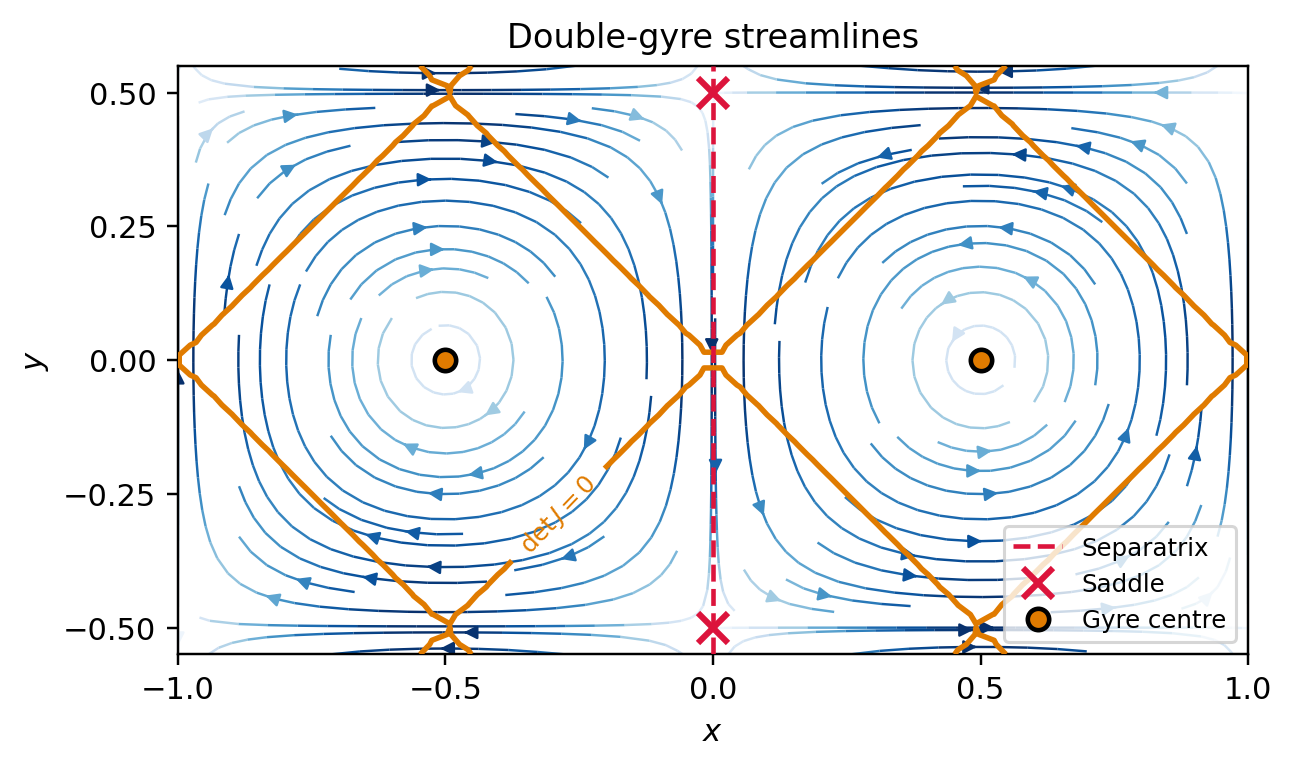
\includegraphics[width=0.45\textwidth]{figures/double_gyre_streamlines.png}
    % TODO: generate with double_gyre_static from
    %   src/fields/environments/Double_Gyre.py.
    % Show: streamlines, separatrix at x=0, saddle points at (0, pm 0.5),
    %   gyre centers at (pm 0.5, 0), det(J)=0 closed contours overlaid.
    \caption{Double-gyre vector field (static case, $A = 0.1$). Streamlines are
    shown in gray. The separatrix at $x = 0$ is shown as a dashed vertical line.
    Saddle points ($\times$) lie at $(0, \pm 0.5)$; gyre centers ($\bullet$) at
    $(\pm 0.5, 0)$. The $\det(\mathbf{J}) = 0$ boundary (solid curve) encloses
    each gyre.}
    \label{fig:dg_streamlines}
\end{figure}

\subsection{Jacobian, $\det(\mathbf{J})$, and the Okubo-Weiss Parameter}

The Jacobian of the vector field evaluated at position $\mathbf{p}$ is
\begin{equation}
    \mathbf{J}(\mathbf{p}) =
    \begin{bmatrix}
        \partial u / \partial x & \partial u / \partial y \\
        \partial v / \partial x & \partial v / \partial y
    \end{bmatrix}
    =
    \begin{bmatrix} a & b \\ d & e \end{bmatrix}. \label{eq:jacobian}
\end{equation}
Its determinant is $\det(\mathbf{J}) = ae - bd$. The Okubo-Weiss parameter $Q$
is related to $\det(\mathbf{J})$ by
\begin{equation}
    Q = \tfrac{1}{4}\bigl(s_n^2 + s_s^2 - \omega^2\bigr) = -\det(\mathbf{J}),
    \label{eq:okubo_weiss}
\end{equation}
where $s_n = \partial u/\partial x - \partial v / \partial y$ is the normal strain
rate, $s_s = \partial v / \partial x + \partial u / \partial y$ is the shear
strain rate, and $\omega = \partial v/\partial x - \partial u/\partial y$ is
twice the local vorticity. The sign convention used throughout this paper is
that $\det(\mathbf{J}) > 0$ characterizes rotation-dominated (vortex-type)
regions and $\det(\mathbf{J}) < 0$ characterizes strain-dominated (hyperbolic)
regions.

Closed-form analytic expressions for $\mathbf{J}(\mathbf{p})$,
$\det(\mathbf{J})(\mathbf{p})$, $\nabla \det(\mathbf{J})(\mathbf{p})$,
$\mathbf{H}_D(\mathbf{p})$, and $Q(\mathbf{p})$ for the static double gyre are
derived in Appendix~\ref{app:analytic}.

\subsection{The $\det(\mathbf{J}) = 0$ Boundary}

The locus $\{\mathbf{p} : \det(\mathbf{J}(\mathbf{p})) = 0\}$ forms two closed
curves in the domain, one encircling each gyre center, separating the
rotation-dominated interior from the strain-dominated exterior.

\begin{figure}[!t]
    \centering
    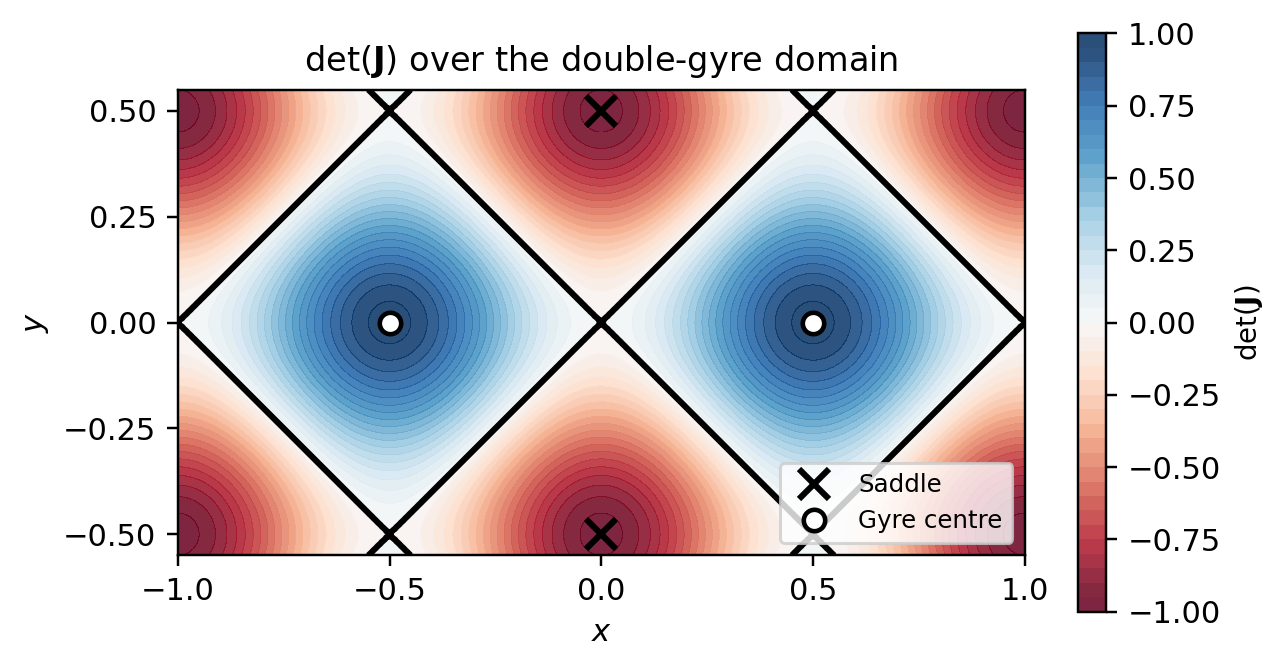
\includegraphics[width=0.45\textwidth]{figures/detJ_contour.png}
    % TODO: generate contour plot of det(J) from the analytic formulas in
    %   Appendix A. Overlay the zero contour in bold. Mark the two saddle
    %   points and the two gyre centers.
    \caption{$\det(\mathbf{J})$ over the double-gyre domain ($A = 0.1$). The
    $\det(\mathbf{J}) = 0$ contour (bold) separates rotation-dominated regions
    (positive, blue) from strain-dominated regions (negative, red). Saddle
    points ($\times$) have strongly negative $\det(\mathbf{J})$.}
    \label{fig:detJ_contour}
\end{figure}

\subsection{Eigenvalue Interpretation}

The sign of $\det(\mathbf{J})$ determines the eigenvalue structure of
$\mathbf{J}$. When $\det(\mathbf{J}) > 0$, the eigenvalues of $\mathbf{J}$
form a complex conjugate pair $\alpha_{\text{eig}} \pm i\omega$ (the flow is
locally rotating); when $\det(\mathbf{J}) < 0$ the eigenvalues are real and
opposite in sign (locally hyperbolic, i.e., saddle-type). The $\det(\mathbf{J})
= 0$ boundary is thus the transition curve between these two topological
regimes.

% Note on alpha collision: alpha_eig denotes the real part of a complex
% eigenvalue pair, i.e., the eigenvalue real part from the Jacobian. It is
% distinct from alpha_mom = exp(-dt/tau), the robot momentum coefficient used
% in Section~\ref{sec:methods}. Both symbols are used in this paper; the
% subscript disambiguates them.


% ---------------------------------------------------------------------------
\section{The Separatrix and Its Relation to the Eulerian Trench}
\label{sec:separatrix}

\subsection{Definition and Location}

The separatrix of the static double gyre is the stable manifold of the two
saddle points $\mathbf{p}^*_1 = (0, -0.5)$ and $\mathbf{p}^*_2 = (0, 0.5)$.
For the static case ($\varepsilon = 0$) this manifold coincides exactly with
the line $x = 0$: trajectories starting on $x = 0$ (except at the saddle
points themselves) converge to one of the two saddle points as $t \to \infty$.
In the time-varying case the separatrix would become a material curve that
evolves with the flow; tracking it would require Lagrangian information.
This paper restricts attention to the static case.

\subsection{The Eulerian Trench in $|\det(\mathbf{J})|$}

Along the separatrix $x = 0$, the local flow is strongly hyperbolic: one
eigenvalue of $\mathbf{J}$ is positive and one is negative, so
$\det(\mathbf{J}) < 0$ and its magnitude is locally large. Moving away from
the separatrix in the $x$-direction into one of the gyres, $\det(\mathbf{J})$
changes sign as the flow becomes rotation-dominated. Consequently, the zero
crossing of $\det(\mathbf{J})$ flanks the separatrix on both sides, and
$|\det(\mathbf{J})|$ has a local minimum (a trench) in the $x$-direction along
the separatrix.

\begin{figure}[!t]
    \centering
    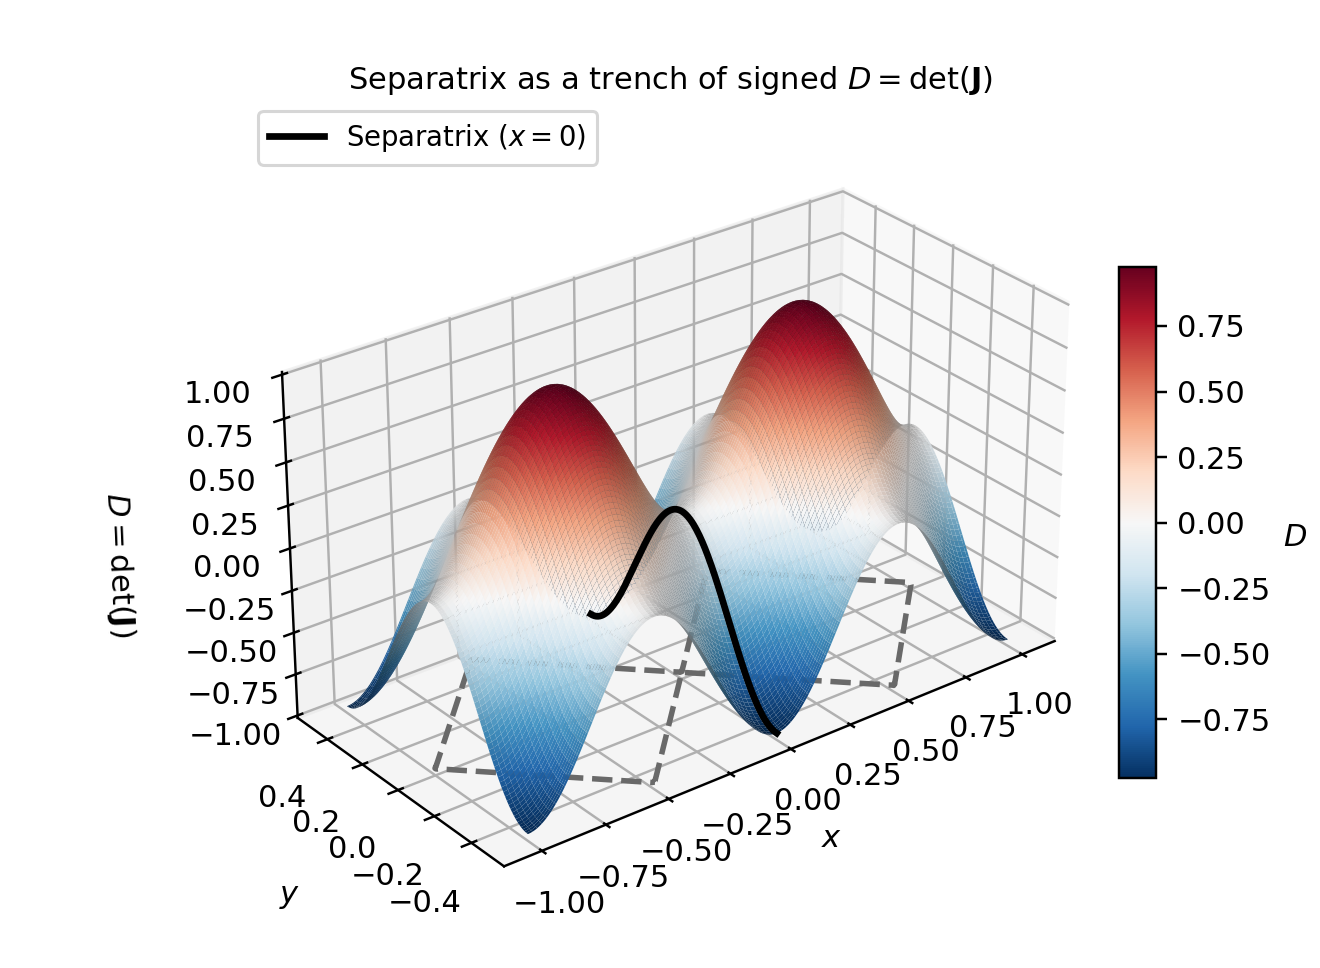
\includegraphics[width=0.45\textwidth]{figures/detJ_trench_cross_section.png}
    % TODO: plot |det(J)| along a horizontal cross-section (fixed y, sweep x)
    % for several values of y (y=0, y=0.2, y=0.4). Show the trench minimum at
    % x=0. Use the analytic det(J) from Appendix A.
    \caption{$|\det(\mathbf{J})|$ along horizontal cross-sections of the double
    gyre at $y = 0$, $0.2$, and $0.4$. The minimum at $x = 0$ (the separatrix)
    defines the Eulerian trench. The minimum deepens as $y \to \pm 0.5$
    (toward the saddle points).}
    \label{fig:trench_cross}
\end{figure}

\subsection{Implications for Navigation}

Because the trench in $|\det(\mathbf{J})|$ aligns with the separatrix, a robot
team that can estimate $\nabla\det(\mathbf{J})$ and $\mathbf{H}_D$ at its
centroid can navigate toward the separatrix by descending into the trench and
then slide along it using the eigenbasis of $\mathbf{H}_D$, without ever
computing a Lagrangian trajectory. This observation motivates the separatrix
controller in Section~\ref{sec:controllers}.


% ---------------------------------------------------------------------------
\section{Distributed Estimation from Six Robots}
\label{sec:estimation}

\subsection{Why Six Robots}

A second-order polynomial in two variables $\phi(x, y) = c_0 + c_1 x + c_2 y
+ c_3 x^2 + c_4 xy + c_5 y^2$ has exactly six coefficients. Fitting the
$u$-component of the field requires solving for $\boldsymbol{\theta}_u =
[c_0, \ldots, c_5]^\top$ from six simultaneous samples; fitting the
$v$-component independently requires the same six. With six robots at distinct
positions in general position, each system is exactly determined. Fewer robots
leave the system underdetermined; more allow least-squares overdetermination.
Six is thus the minimum number of robots required to recover a full quadratic
model of both field components simultaneously.

\subsection{Pentagon-of-Pairs Formation}

The six robots are arranged as three pairs. The midpoint of each pair defines
a vertex of a triangle, and the triangle is specified in SAS (side-angle-side)
parameterization with state vector
$(x_c, y_c, \theta_c, p_1, \beta_1, q_1, L_2, \theta_2, L_3, \theta_3,
L_4, \theta_4)$, where $(x_c, y_c)$ is the centroid of the triangle,
$\theta_c$ is its heading, $(p_1, \beta_1, q_1)$ are the SAS parameters of
the triangle, and $(L_k, \theta_k)$ describe the length and orientation of
the $k$-th pair. This formation is implemented in \textit{pentagon\_cluster.py}.

\begin{figure}[!t]
    \centering
    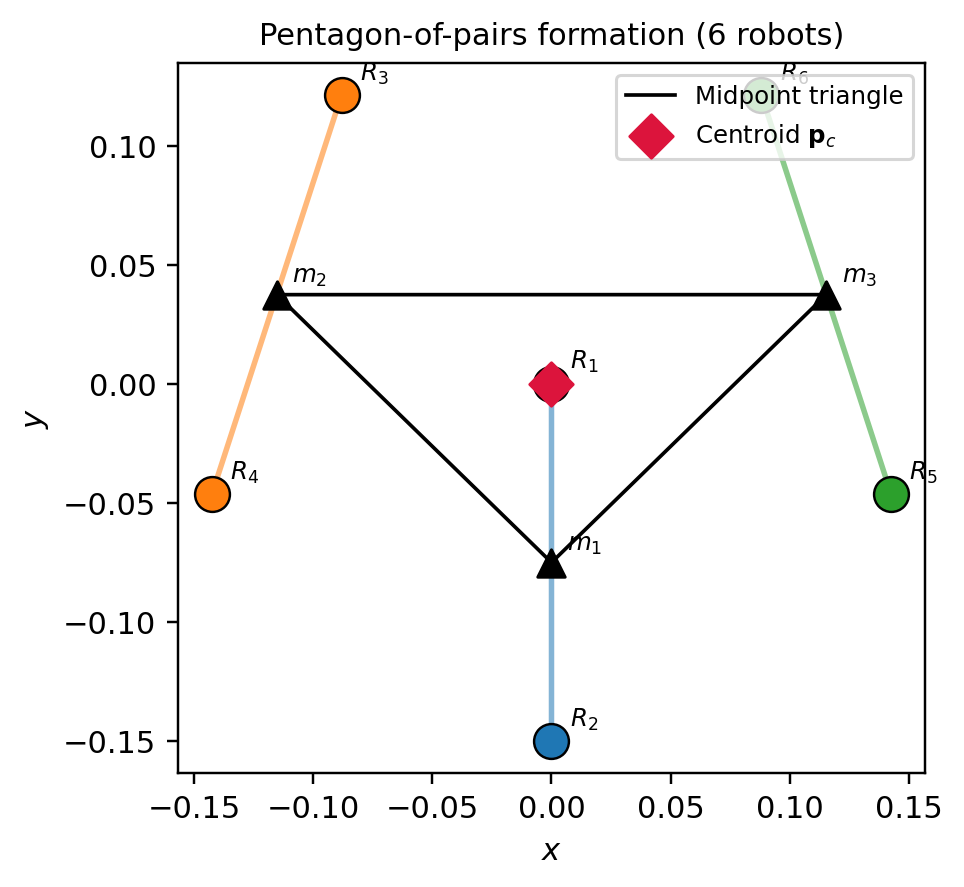
\includegraphics[width=0.40\textwidth]{figures/pentagon_formation.png}
    % TODO: draw the six-robot formation. Show: three pairs with midpoints
    % labeled m1, m2, m3; the SAS triangle formed by the midpoints; the centroid
    % p_c; robots labeled R1-R6. Annotate p_1, beta_1, q_1 and one pair length L.
    \caption{Pentagon-of-pairs formation. Six robots (circles) are arranged in
    three pairs (shaded). The midpoints ($\blacktriangle$) form a triangle
    parameterized by SAS parameters $(p_1, \beta_1, q_1)$. The cluster centroid
    $\mathbf{p}_c$ lies at the centroid of the triangle.}
    \label{fig:pentagon_formation}
\end{figure}

\subsection{Quadratic Estimation of the Vector Field}

Let $\mathbf{p}_i = (x_i, y_i)$, $i = 1, \ldots, 6$ be the robot positions and
let $\tilde{\mathbf{p}}_i = \mathbf{p}_i - \mathbf{p}_c$ be the position of
robot $i$ relative to the centroid. Define the quadratic basis vector for robot
$i$ as
\begin{equation}
    \boldsymbol{\phi}(\tilde{x}_i, \tilde{y}_i) =
    [1, \; \tilde{x}_i, \; \tilde{y}_i, \; \tilde{x}_i^2, \;
    \tilde{x}_i \tilde{y}_i, \; \tilde{y}_i^2]^\top. \label{eq:basis}
\end{equation}
Stacking the six basis vectors forms the $6 \times 6$ design matrix
$\boldsymbol{\Phi}$, with $\boldsymbol{\Phi}_{ij} =
\phi_j(\tilde{x}_i, \tilde{y}_i)$.
The coefficient vectors are obtained by solving
\begin{equation}
    \boldsymbol{\Phi} \boldsymbol{\theta}_u = \mathbf{u}, \quad
    \boldsymbol{\Phi} \boldsymbol{\theta}_v = \mathbf{v}, \label{eq:solve}
\end{equation}
where $\mathbf{u} = [u_1, \ldots, u_6]^\top$ and $\mathbf{v} = [v_1, \ldots,
v_6]^\top$ are the measured field components at the six robot positions. When
$\det(\boldsymbol{\Phi}) \neq 0$ (non-degenerate formation) the system is solved
exactly; otherwise least-squares is used as a fallback.

\subsection{Closed-Form Recovery of $\det(\mathbf{J})$ and Its Derivatives}

Let $\boldsymbol{\theta}_u = [u_c, u_x, u_y, u_{xx}, u_{xy}, u_{yy}]^\top$
and $\boldsymbol{\theta}_v = [v_c, v_x, v_y, v_{xx}, v_{xy}, v_{yy}]^\top$.
The estimated Jacobian at the centroid is
\begin{equation}
    \hat{\mathbf{J}} =
    \begin{bmatrix} u_x & u_y \\ v_x & v_y \end{bmatrix}, \label{eq:J_hat}
\end{equation}
with $\det(\hat{\mathbf{J}}) = u_x v_y - u_y v_x$.

Differentiating $\det(\mathbf{J})(x, y) = (\partial u / \partial x)(\partial v
/ \partial y) - (\partial u / \partial y)(\partial v / \partial x)$ using the
quadratic model gives the gradient at the centroid as
\begin{equation}
    \nabla\det(\hat{\mathbf{J}}) =
    \begin{bmatrix}
        u_{xx} v_y + u_x v_{xy} - u_{xy} v_x - u_y v_{xx} \\
        u_{xy} v_y + u_x v_{yy} - u_{yy} v_x - u_y v_{xy}
    \end{bmatrix}, \label{eq:grad_det}
\end{equation}
and the Hessian $\mathbf{H}_D$ at the centroid as
\begin{equation}
    \mathbf{H}_D =
    \begin{bmatrix}
        2(u_{xx} v_{xy} - u_{xy} v_{xx}) &
        u_{xx} v_{yy} - u_{yy} v_{xx} \\
        u_{xx} v_{yy} - u_{yy} v_{xx} &
        2(u_{xy} v_{yy} - u_{yy} v_{xy})
    \end{bmatrix}. \label{eq:hess_det}
\end{equation}
These expressions are derived algebraically from the quadratic fit coefficients
and require no additional field evaluations beyond the six robot measurements.

\subsection{Conditioning and Degenerate Configurations}

The system~(\ref{eq:solve}) is non-degenerate when $\det(\boldsymbol{\Phi})
\neq 0$, which holds when no four of the six robots are collinear and no two
share the same position. Degenerate configurations arise when the cluster
collapses (formation maintenance failure) or becomes nearly collinear. In
practice the cluster space controller maintains the nominal formation geometry;
the determinant of $\boldsymbol{\Phi}$ is monitored during simulation and the
experiment is logged as failed if it falls below a threshold of $10^{-10}$.


% ---------------------------------------------------------------------------
\section{Adaptive Controllers}
\label{sec:controllers}

\subsection{Common Control Architecture}
\label{sec:arch}

Both controllers follow the same three-layer architecture:

\begin{enumerate}
    \item \textbf{Navigation primitive.} Given the six robot positions and their
          field measurements, compute a centroid velocity command
          $(\dot{x}_c^\text{des}, \dot{y}_c^\text{des})$.
    \item \textbf{Cluster space controller.} Using the 12-state SAS
          parameterization and the $12 \times 12$ inverse kinematic Jacobian
          (Appendix~\ref{app:kinematics}), distribute the centroid velocity
          command to six individual robot velocity commands while maintaining
          the nominal formation shape.
    \item \textbf{Robot dynamics.} Each robot obeys a first-order momentum model
          \begin{equation}
              \mathbf{v}[k+1] = \alpha_{\text{mom}}\,\mathbf{v}[k]
              + (1 - \alpha_{\text{mom}})\,\mathbf{v}^{\text{des}}[k],
              \label{eq:momentum}
          \end{equation}
          where $\alpha_{\text{mom}} = \exp(-\Delta t / \tau)$ with actuator
          time constant $\tau = 0.3$ s and step $\Delta t = 0.1$ s, giving
          $\alpha_{\text{mom}} \approx 0.717$. Velocities are saturated to
          $|\mathbf{v}| \leq v_{\max} = 0.3$ m/s and a stiction floor of
          $v_{\text{stiction}} = 0.05$ m/s is applied.
\end{enumerate}

Note on notation: $\alpha_{\text{mom}}$ denotes the momentum coefficient in
(\ref{eq:momentum}); $\alpha_{\text{eig}}$ (used in
Section~\ref{sec:detj_field}) denotes the real part of a complex eigenvalue
pair of $\mathbf{J}$. These are distinct quantities from different parts of the
system.

\subsection{Controller 1: Separatrix Tracker (Logic C)}
\label{sec:sep_controller}

The separatrix tracker navigates the cluster centroid toward and then along
the separatrix of the double gyre by operating in three modes: FLOW (on the
separatrix), Logic A (attract toward the trench), and Logic B (slide along
the trench). Mode selection uses the eigenbasis of $\mathbf{H}_D$ and the
local field vector $\mathbf{f} = (u_c, v_c)$ at the centroid.

Let $\lambda_{\min}$, $\mathbf{v}_-$ denote the most negative eigenvalue and
its eigenvector (the along-trench direction), and $\lambda_{\max}$,
$\mathbf{v}_+$ the most positive eigenvalue and its eigenvector (the
cross-trench direction). The cluster is declared to be on the separatrix
(in the FLOW band) when either
\begin{equation}
    |\det(\hat{\mathbf{J}})| < \varepsilon_{\text{raw}}, \quad
    \text{or} \quad
    \frac{|\det(\hat{\mathbf{J}})|}{||\mathbf{H}_D||_F} < \varepsilon_{\text{dim}},
    \label{eq:flow_band}
\end{equation}
where $\varepsilon_{\text{raw}} = 10^{-3}$ and $\varepsilon_{\text{dim}} =
0.025$ are the raw and dimensionless thresholds. The second condition normalizes
by the Frobenius norm of $\mathbf{H}_D$ to make the test scale-invariant.

\vspace{4pt}
\noindent\textbf{Algorithm 1: Logic C Separatrix Tracker}
\begin{algorithmic}[1]
    \STATE \textbf{Parameters:} $v_{\max}$, $\varepsilon_{\text{raw}}$,
           $\varepsilon_{\text{dim}}$
    \STATE \textbf{Input:} cluster positions $\{\mathbf{p}_i\}$,
           measurements $\{(u_i, v_i)\}$
    \STATE \textbf{Output:} centroid velocity command $(v_{x,c}, v_{y,c})$
    \STATE Solve~(\ref{eq:solve}) to obtain $\boldsymbol{\theta}_u$,
           $\boldsymbol{\theta}_v$
    \STATE Compute $D \leftarrow \det(\hat{\mathbf{J}})$ via~(\ref{eq:J_hat}),
           $\mathbf{g} \leftarrow \nabla\det(\hat{\mathbf{J}})$
           via~(\ref{eq:grad_det}),
           $\mathbf{H}_D$ via~(\ref{eq:hess_det})
    \STATE Compute $\mathbf{f} \leftarrow (u_c, v_c)$ (field at centroid)
    \IF{$|D| < \varepsilon_{\text{raw}}$ \textbf{or}
        $|D| / \|\mathbf{H}_D\|_F < \varepsilon_{\text{dim}}$}
        \STATE \textit{// FLOW mode: on separatrix}
        \STATE Eigendecompose $\mathbf{H}_D \to (\lambda_{\min}, \mathbf{v}_-)$,
               $(\lambda_{\max}, \mathbf{v}_+)$
        \STATE $c_{\text{along}} \leftarrow \mathbf{f}^\top \mathbf{v}_-$
        \STATE $r_{\perp} \leftarrow (\mathbf{g}^\top \mathbf{v}_+) /
               \lambda_{\max}$; \; $c_{\perp} \leftarrow -r_{\perp}$
        \STATE $\boldsymbol{\delta} \leftarrow v_{\max}\tanh(c_{\text{along}} /
               v_{\max})\,\mathbf{v}_- + v_{\max}\tanh(c_{\perp} /
               v_{\max})\,\mathbf{v}_+$
    \ELSE
        \STATE Eigendecompose $\mathbf{H}_D$; let $\mathbf{v}_-$ point in
               direction of decreasing $D$
        \IF{$\mathbf{f}^\top \mathbf{v}_- > 0$}
            \STATE \textit{// Logic B: flow along trench descent}
            \STATE $c_k \leftarrow -(\mathbf{v}_k^\top \mathbf{g}) /
                   |\lambda_k|$ for $k \in \{-, +\}$
        \ELSE
            \STATE \textit{// Logic A: attract toward saddle}
            \STATE $c_k \leftarrow -(\mathbf{v}_k^\top \mathbf{g}) /
                   \lambda_k$ for $k \in \{-, +\}$
        \ENDIF
        \STATE $\boldsymbol{\delta} \leftarrow
               \sum_{k} v_{\max}\tanh(c_k / v_{\max})\,\mathbf{v}_k$
    \ENDIF
    \RETURN $(v_{x,c}, v_{y,c}) \leftarrow (\delta_x, \delta_y)$
\end{algorithmic}

\vspace{4pt}

This controller is implemented as \textit{separatrix\_logic\_c\_step} in
\textit{pentagon\_primitives.py} (lines 420-511).

\subsection{Controller 2: Okubo-Weiss Boundary Tracker}
\label{sec:ow_controller}

The Okubo-Weiss boundary tracker drives the cluster centroid to the
$\det(\mathbf{J}) = 0$ contour using a Newton step in the perpendicular
direction and drifts tangentially along the contour using the smallest-magnitude
eigenvector of $\mathbf{H}_D$.

\vspace{4pt}
\noindent\textbf{Algorithm 2: Newton-Step Okubo-Weiss Boundary Tracker}
\begin{algorithmic}[1]
    \STATE \textbf{Parameters:} $v_{\max}$, $\varepsilon_{\text{grad}}$
           (gradient norm fallback threshold)
    \STATE \textbf{Input:} cluster positions $\{\mathbf{p}_i\}$,
           measurements $\{(u_i, v_i)\}$
    \STATE \textbf{Output:} centroid velocity command $(v_{x,c}, v_{y,c})$
    \STATE Compute $D$, $\mathbf{g}$, $\mathbf{H}_D$, $\mathbf{f}$ as in
           Steps 4-6 of Algorithm 1
    \STATE $g_{\text{norm}} \leftarrow \|\mathbf{g}\|$
    \IF{$g_{\text{norm}} < \varepsilon_{\text{grad}}$}
        \STATE \textit{// Degenerate fallback: drift with flow}
        \STATE $\boldsymbol{\delta} \leftarrow
               v_{\max}\tanh(||\mathbf{f}|| / v_{\max}) \cdot
               \mathbf{f} / ||\mathbf{f}||$
        \RETURN $(\delta_x, \delta_y)$
    \ENDIF
    \STATE \textit{// Perpendicular Newton step toward $D = 0$}
    \STATE $\Delta \mathbf{p}_{\perp} \leftarrow
           -(D / g_{\text{norm}}^2)\,\mathbf{g}$
    \STATE $\hat{\mathbf{u}} \leftarrow -\text{sign}(D)\,\mathbf{g} /
           g_{\text{norm}}$
    \STATE $c_{\perp} \leftarrow \Delta\mathbf{p}_{\perp}^\top \hat{\mathbf{u}}$
    \STATE $s_{\perp} \leftarrow v_{\max}\tanh(c_{\perp} / v_{\max})$
    \STATE \textit{// Tangential drift along contour}
    \STATE Eigendecompose $\mathbf{H}_D$; let $i_{\tan} =
           \arg\min_k |\lambda_k|$; $\mathbf{v}_{\tan} \leftarrow
           V[:, i_{\tan}]$
    \STATE Sign-stabilize: if $\mathbf{f}^\top \mathbf{v}_{\tan} < 0$ then
           $\mathbf{v}_{\tan} \leftarrow -\mathbf{v}_{\tan}$
    \STATE $c_{\tan} \leftarrow \mathbf{f}^\top \mathbf{v}_{\tan}$; \;
           $s_{\tan} \leftarrow v_{\max}\tanh(c_{\tan} / v_{\max})$
    \STATE $\boldsymbol{\delta} \leftarrow s_{\perp}\hat{\mathbf{u}} +
           s_{\tan}\mathbf{v}_{\tan}$
    \RETURN $(v_{x,c}, v_{y,c}) \leftarrow (\delta_x, \delta_y)$
\end{algorithmic}

\vspace{4pt}

This controller is implemented as \textit{logic\_g\_newton\_contour\_pentagon}
in \textit{pentagon\_primitives.py} (lines 612-689).

\subsection{Gain Selection and Velocity Limits}

Both controllers use the same saturation structure: $v_{\max}\tanh(c /
v_{\max})$ saturates smoothly at $\pm v_{\max}$. The parameters
$v_{\max} = 0.04$ m/s (primitive-level saturation speed),
$v_{\text{stiction}} = 0.05$ m/s, and $v_{\text{max,robot}} = 0.3$ m/s
are fixed throughout all simulations. The FLOW-band thresholds
$\varepsilon_{\text{raw}} = 10^{-3}$ and $\varepsilon_{\text{dim}} = 0.025$
are the values from the implementation and are fixed unless otherwise noted.

% TODO: add a table of all parameters here (mirror Table I style from
%   Paper_Draft_3A.tex): columns for symbol, value, units, description.
% Include: v_max, v_stiction, v_max_robot, alpha_mom, tau, dt, A (amplitude),
% eps_raw, eps_dim, eps_grad.


% ---------------------------------------------------------------------------
\section{Stability Analysis}
\label{sec:stability}

\subsection{Okubo-Weiss Boundary Controller}
\label{sec:stab_ow}

\textbf{Lyapunov candidate.} Define $V_1 = \tfrac{1}{2} D^2$ where
$D = \det(\mathbf{J}(\mathbf{p}_c))$ and $\mathbf{p}_c$ is the cluster
centroid.

\textbf{Time derivative.} Along continuous-time trajectories,
\begin{equation}
    \dot{V}_1 = D \, \nabla D^\top \dot{\mathbf{p}}_c. \label{eq:V1dot}
\end{equation}
Under the Newton-step control law the commanded centroid velocity is
$\dot{\mathbf{p}}_c^{\text{des}} = \Delta\mathbf{p}_{\perp} = -(D /
\|\mathbf{g}\|^2)\,\mathbf{g}$. Substituting into~(\ref{eq:V1dot}) and
ignoring the tangential component (which is orthogonal to $\mathbf{g}$):
\begin{equation}
    \dot{V}_1 = D \, \mathbf{g}^\top \left(- \frac{D}{\|\mathbf{g}\|^2}
    \mathbf{g}\right) = -\frac{D^2 \|\mathbf{g}\|^2}{\|\mathbf{g}\|^2}
    = -D^2. \label{eq:V1dot_clean}
\end{equation}
Thus $\dot{V}_1 = -D^2 = -2V_1 \leq 0$, with $\dot{V}_1 = 0$ if and only if
$D = 0$.

% TODO: verify the algebra above. Note the saturation via tanh introduces a
% bounded deviation; the following robustness statement needs to account for it.

\textbf{Convergence basin.} $V_1$ is globally defined and $\dot{V}_1 \leq 0$
everywhere (in the noise-free, unsaturated case), so $D(t) \to 0$ from any
initial condition with $D(0)$ finite. The saturation via $\tanh$ modifies this:

% TODO: state formally that the tanh modification gives V1_dot = -k_s * D^2
% where k_s = tanh(c_perp / v_max) / c_perp in (0, 1] by properties of tanh.
% Thus V1_dot <= 0 still holds globally; only the convergence rate is reduced
% near saturation.

\textbf{Robustness under measurement noise.} Suppose each robot's field
measurement is corrupted by additive noise: $u_i^m = u(\mathbf{p}_i) + \eta_i^u$,
$v_i^m = v(\mathbf{p}_i) + \eta_i^v$, with $|\eta| \leq \bar{\eta}$.
The estimated determinant satisfies $\hat{D} = D + \epsilon_D$ where the
estimation error $\epsilon_D$ is bounded by
\begin{equation}
    |\epsilon_D| \leq C_J(\boldsymbol{\Phi})\,\bar{\eta}, \label{eq:noise_bound}
\end{equation}
and $C_J(\boldsymbol{\Phi})$ is a conditioning constant that depends on the
formation geometry through the design matrix $\boldsymbol{\Phi}$.

% TODO: derive the explicit bound on C_J. It involves the condition number of
% Phi and the magnitude of the Jacobian first-order coefficients. This is the
% ISS-style robustness result: the ultimate bound on D(t) scales as
% C_J * eta_bar under persistent noise.

\subsection{Separatrix Tracker}
\label{sec:stab_sep}

\textbf{Lyapunov candidate.} Define
\begin{equation}
    V_2 = \tfrac{1}{2}\bigl(\mathbf{g}^\top \mathbf{v}_-\bigr)^2
          + \tfrac{w}{2} D^2, \label{eq:V2}
\end{equation}
where $\mathbf{v}_-$ is the along-trench eigenvector of $\mathbf{H}_D$ (the
eigenvector corresponding to $\lambda_{\min}$, normalized), $\mathbf{g} =
\nabla\det(\mathbf{J})$, and $w > 0$ is a positive weighting constant.
The first term measures how much the gradient of $\det(\mathbf{J})$ points
in the along-trench direction (which should vanish on the separatrix trench
minimum); the second term penalizes distance from $D = 0$.

% TODO: this is the proposed Lyapunov candidate; verify it is appropriate
% for the Logic C hybrid structure. The main challenge is handling
% V2_dot at mode boundaries.

\textbf{FLOW mode ($|D| < \varepsilon_{\text{raw}}$ or dimensionless threshold).}
In FLOW mode the centroid moves along $\mathbf{v}_-$ and snaps back toward
$D = 0$ along $\mathbf{v}_+$. Show that the $\mathbf{v}_+$ (cross-trench)
snap drives $D \to 0$, contributing $-w D^2$ to $\dot{V}_2$ from the second
term. The along-trench component does not change $D$ to first order, so its
contribution to the second term is zero. The first term...

% TODO: complete the FLOW-mode V2_dot derivation. Show the along-trench
% component does not increase (g^T v_neg)^2 because the slide is along v_neg.
% The snap along v_pos reduces (g^T v_neg)^2 if H_D has the right sign structure
% near the trench minimum. This requires a local second-order argument.

\textbf{Logic A mode (attract toward trench).}

% TODO: show that Logic A (Newton step in the signed-lambda basis of H_D)
% acts as a gradient descent on V2. The signed-lambda denominator gives
% descent in all directions of H_D simultaneously. Derive V2_dot <= 0 for
% this mode.

\textbf{Logic B mode (slide along trench descent).}

% TODO: show that Logic B (|lambda| denominator) reduces the along-trench
% gradient component while keeping the cross-trench component. Derive
% V2_dot behavior.

\textbf{Hybrid argument.}

% TODO: state a dwell-time assumption (minimum time in each mode). Use a
% common Lyapunov function argument: V2 is continuous across mode switches
% (it does not depend on which mode is active). Show that the total
% decrease in V2 over a bounded sequence of mode switches is negative if
% each mode is active for at least a minimum dwell time. This gives
% practical stability of the separatrix (V2 converges to a residual
% determined by the noise bound and the dwell time).

\subsection{ISS-Style Robustness}
\label{sec:stab_iss}

% TODO: state the ISS (input-to-state stability) bound for both controllers
% under bounded additive noise (u_meas = u_true + N(0, sigma^2) per robot).
% The bound takes the form: the ultimate bound on |D(t)| (for the OW
% controller) or on V2(t) (for the separatrix controller) scales linearly
% with sigma_uv * C_cond, where C_cond is a formation-geometry-dependent
% conditioning constant. State the main result as a proposition, with the
% full proof deferred to a cited technical report or appendix.


% ---------------------------------------------------------------------------
\section{Methods}
\label{sec:methods}

\subsection{Cluster Space Controller and SAS Formation}

Both controllers use the same underlying cluster space controller and
pentagon-of-pairs formation. The forward kinematics maps the 12-state
cluster configuration to global robot positions; the inverse kinematics
and analytic $12 \times 12$ inverse kinematic Jacobian (see
Appendix~\ref{app:kinematics}) map a desired centroid velocity to
individual robot velocity commands while maintaining nominal pair lengths
and the SAS triangle shape.

Formation maintenance gains are set to...
% TODO: state the gain values used for formation maintenance in
% pentagon_cluster.py (proportional gain on each shape error term).
% Verify against pentagon_cluster.py lines 165-167.

\subsection{Six-Robot Configuration}

% TODO: fill in the specific initial side lengths (p_1, beta_1, q_1), pair
% lengths (L_2, L_3, L_4), and initial heading used for all simulation trials.
% These are the nominal formation parameters. State the centroid placement
% rule (e.g., centroid starts at the first point in the initial-condition grid).

\subsection{Simulation Program}

Simulations are run using the Python framework in the
\textit{trunk/Python_Simulations/Vector\_Fields/VF\_Robot/} directory.
The field is the static double gyre (\textit{double\_gyre\_static},
amplitude $A = 0.1$) on the domain $[-1, 1] \times [-0.5, 0.5]$. The
integrator is explicit Euler at 10 Hz ($\Delta t = 0.1$ s). Robot dynamics
follow the first-order model~(\ref{eq:momentum}) with $\tau = 0.3$ s. Each
trial runs for 200 steps (20 s). The separatrix controller experiment uses
\textit{experiments/main\_separatrix\_v6r.py}; the Okubo-Weiss controller
uses \textit{experiments/main\_logic\_g\_newton\_pentagon.py}.

\subsection{Ocean HFR Simulation}
\label{sec:ocean_sim}

% --- DATA PROVENANCE AND REPRODUCTION INSTRUCTIONS ---
% The 29 NetCDF files used here are the USWC Radial-to-Total Vector (RTV)
% product at 6 km resolution, produced by CORDC/Scripps and archived at NOAA
% NCEI under accession gov.noaa.nodc:IOOS-HFRadarRTVector.
%
% To re-download the exact 29 hourly files used in this experiment:
%
%   BASE=https://www.ncei.noaa.gov/thredds-ocean/fileServer/ioos/hfradar/rtv/2012/201205/USWC
%
%   for HOUR in 0800 0900 1000 1100 1200 1300 1400 1500 1600 1700 \
%               1800 1900 2000 2100 2200 2300 0000 0100 0200 0300 \
%               0400 0500 0600 0700 0800 0900 1000 1100 1200; do
%     # May 16 files use date prefix 20120516; May 17 files use 20120517.
%     # Hours 0800-2300 on May 16 are prefix 201205160800 through 201205162300.
%     # Hours 0000-1200 on May 17 are prefix 201205170000 through 201205171200.
%     curl -O "$BASE/${TIMESTAMP}_hfr_uswc_6km_rtv_uwls_SIO.nc"
%   done
%
% Construct TIMESTAMP as YYYYMMDDHHOO where YYYYMMDD is the calendar date and
% HHOO is the UTC hour plus two zero digits (e.g., 201205160800 for
% May 16 08:00 UTC). The server returns HTTP 200 directly; no authentication
% or browser session is required.  The files were originally batch-exported
% from the CORDC internal archive on 2020-01-21 by user "motero" using the
% tool rtvUpdateNetcdf (visible in each file's NC history attribute).
% The UCSD/Scripps THREDDS server (hfrnet-tds.ucsd.edu) was decommissioned
% June 30, 2025; do not attempt to use it.
%
% A 2 km resolution version of the same 29 hours is available at the same
% NCEI path with the token "2km" in place of "6km".  See
% trunk/Python_Simulations/Vector_Fields/ocean_data/DATA_PROVENANCE.md
% for a full inventory and notes on spatial coverage differences.
% --- END DATA PROVENANCE ---

The ocean experiment uses hourly surface-current frames from the
Santa Barbara Channel HF radar archive (May 16--17, 2012, 29 hourly
frames covering 28~h of real time). The data are the U.S.~West~Coast
Radial-to-Total Vector (RTV) product produced by the Scripps Coastal
Ocean Observing Laboratory (CORDC) HFRNet network and archived at the
NOAA National Centers for Environmental Information under accession
\texttt{gov.noaa.nodc:IOOS-HFRadarRTVector}, retrieved from the NOAA
THREDDS-Ocean server in June 2026. The 6~km resolution files were
used; each file contains one hour of surface-current velocity
components ($u$, $v$) on a regular geographic grid. Frames are linearly interpolated
in time inside the field evaluator
(\textit{ocean\_hfr\_socal\_timevarying} in
\textit{src/fields/environments/Ocean\_HFR.py}). The cluster runs in
non-dimensional world coordinates on $[-0.65, 0.65]^2$, and an affine
map carries those coordinates to a geographic region of radius
$0.3^{\circ}$ centered on $(34.2^{\circ}\mathrm{N},
-120.4^{\circ}\mathrm{W})$. One world unit therefore corresponds to
approximately $51$ km of latitude at this center.

The simulator's discrete-time step is treated as one sample per ten
minutes of real time, rather than the testbed's native $0.1$ s. Under
this interpretation, the cluster's steady-state command magnitude
($V_{\max} \cdot k = 0.04 \cdot 3.0 = 0.12$ world units per step) maps
to a geographic centroid speed of approximately
$0.12 \cdot 51 \mathrm{\,km} / 600 \mathrm{\,s} \approx 1$ m/s,
consistent with the survey speed of a small autonomous surface vessel.
The momentum filter (Eq.~\ref{eq:momentum}) with $\alpha = 0.7$ then
corresponds to a maneuvering time constant of
$\tau = -600 / \ln(0.7) \approx 28$ min, which is a physically
reasonable inertia for an ASV maneuvering against ocean current
loading. With this relabeling, $110$ sample steps span
$110 \cdot 10$ min $= 18.3$ h of real field time and traverse
approximately $18$ of the $29$ HFR frames. The cluster therefore
operates as a slow Lagrangian-scale tracer being actively steered
against an evolving background current.

The motor-friction stiction floor used in the testbed model
(\textit{STICTION\_THRESHOLD} $= 0.025$ world units per step in
\textit{omnibot.py}) is retained but does not activate at the chosen
operating point. We note this floor is a leftover from the laboratory
model and is not physically meaningful for a vessel-scale platform; it
simply prescribes a lower-bound cutoff on commanded centroid velocity
of approximately $0.21$ m/s.

\subsection{Noise Model}

Measurement noise is additive Gaussian on the $(u, v)$ components at each
robot position:
\begin{equation}
    u_i^m = u(\mathbf{p}_i) + \eta_i^u, \quad
    v_i^m = v(\mathbf{p}_i) + \eta_i^v,
    \quad \eta \sim \mathcal{N}(0, \sigma_{uv}^2),
    \label{eq:meas_noise}
\end{equation}
with noise samples independent across robots and time steps. Position noise
is additive Gaussian on each robot's reported position:
\begin{equation}
    \mathbf{p}_i^m = \mathbf{p}_i + \boldsymbol{\xi}_i, \quad
    \boldsymbol{\xi}_i \sim \mathcal{N}(\mathbf{0}, \sigma_p^2 \mathbf{I}).
    \label{eq:pos_noise}
\end{equation}

Both noise hooks must be implemented before the sweeps described in
Section~\ref{sec:test_plan} can be run. Measurement noise (\ref{eq:meas_noise})
follows the existing precedent in \textit{src/fields/field\_types.py}
(\textit{NNField}, \textit{RBFField}, \textit{EnsembleField} each accept a
\textit{noise\_std} parameter); it requires adding a \textit{noise\_std}
argument to the \textit{AnalyticalField} class or to the primitive's
\textit{\_sample\_vector\_at\_robots} function. Position noise
(\ref{eq:pos_noise}) has no current precedent in the simulator; it requires
a new hook in the cluster state update.

\subsection{Testing Plan}
\label{sec:test_plan}

Both controllers are evaluated over the following sweep:
\begin{itemize}
    \item $\sigma_{uv} \in \{0,\; 0.001,\; 0.005,\; 0.01,\; 0.02,\; 0.05\}$
          (m/s, measurement noise standard deviation).
    \item $\sigma_p \in \{0,\; 0.005,\; 0.01,\; 0.02\}$ m
          (position noise standard deviation).
    \item Initial centroid: $5 \times 5$ uniform grid over
          $[-0.8, 0.8] \times [-0.8, 0.8]$, plus 25 random centroids per
          cell ($N = 200$ trials per noise cell in total).
    \item Initial cluster heading: uniformly random in $[0, 2\pi)$.
\end{itemize}

The following metrics are recorded for each trial:
\begin{enumerate}
    \item \textbf{Time-to-band:} the first step at which the quantity of
          interest (for the OW controller, $|\det(\mathbf{J}(\mathbf{p}_c))|$;
          for the separatrix controller, the $x$-distance from the separatrix
          $|x_c|$) drops below a threshold and remains below it for at least
          10 consecutive steps.
    \item \textbf{Tracking error:} mean and 95th percentile of the tracking
          quantity over steps 100-200 (the tracking phase after transient
          convergence).
    \item \textbf{Formation shape error:} RMS deviation of the six robot
          positions from their nominal positions at the given cluster centroid.
    \item \textbf{Control effort:} $\int_0^T \|\mathbf{v}^{\text{des}}(t)\|
          \,dt$ over the trial.
\end{enumerate}

A trial is declared successful if metric (1) is achieved within 200 steps
without formation collapse (shape error exceeds twice the nominal pair
length). Success rates are reported as the fraction of successful trials
in each $(\sigma_{uv}, \sigma_p)$ cell.


% ---------------------------------------------------------------------------
\section{Results}
\label{sec:results}

\subsection{Estimator Accuracy versus Noise}

\begin{figure}[!t]
    \centering
    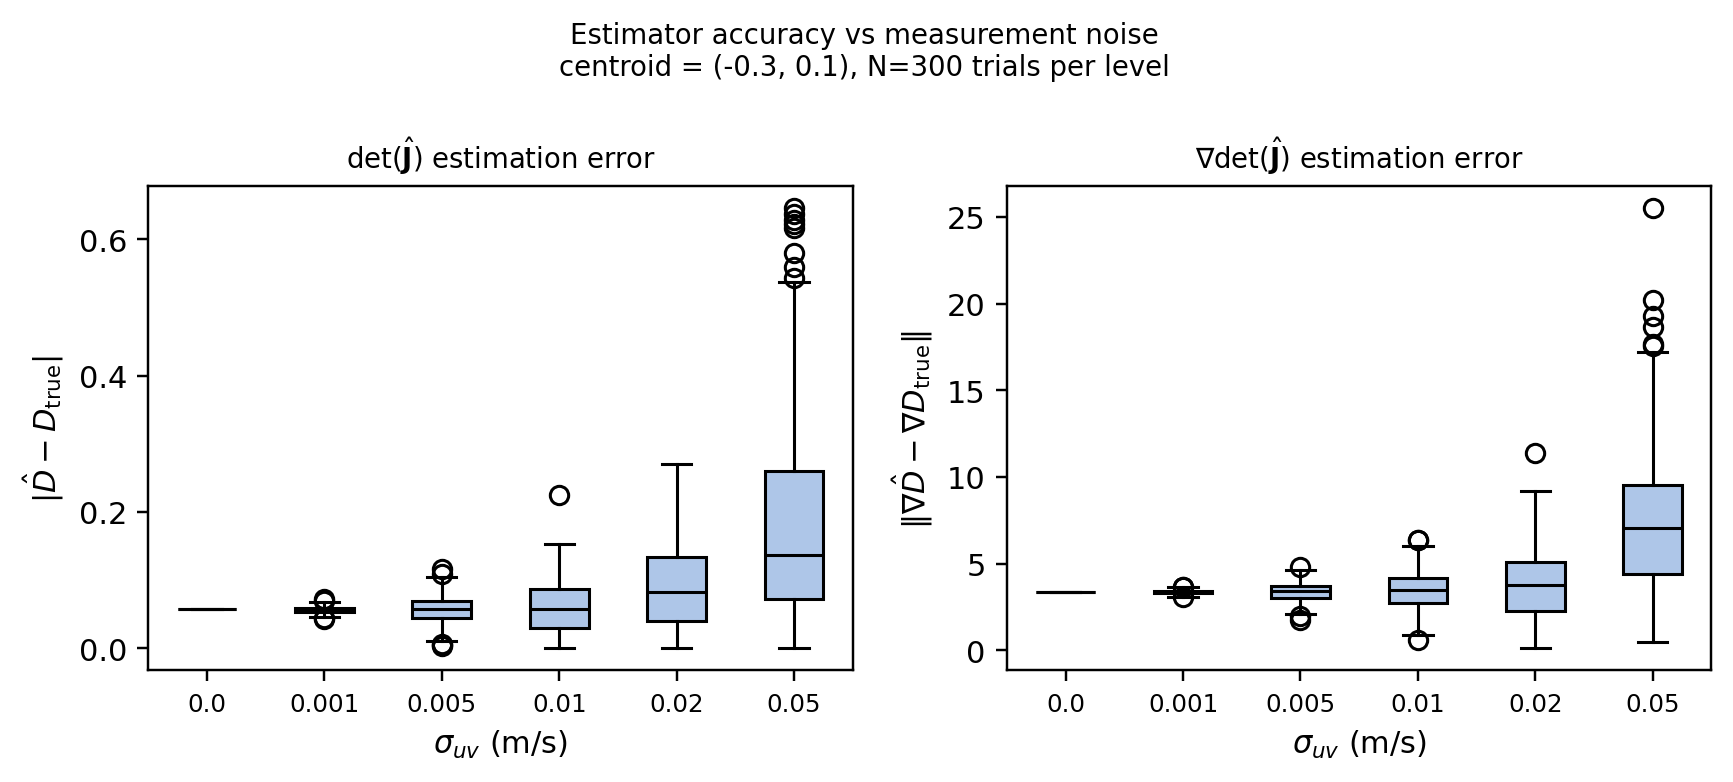
\includegraphics[width=0.45\textwidth]{figures/estimator_accuracy_vs_noise.png}
    % TODO: plot estimation error (|D_hat - D_true|, |grad_D_hat - grad_D_true|)
    % vs sigma_uv at fixed formation size, then vs formation size at fixed sigma.
    % Use box plots over Monte Carlo runs.
    \caption{Estimation error of $\det(\hat{\mathbf{J}})$ and
    $\|\nabla\det(\hat{\mathbf{J}}) - \nabla\det(\mathbf{J})\|$ as a function
    of measurement noise standard deviation $\sigma_{uv}$, with the nominal
    formation size. Boxes show median, quartiles, and 1.5$\times$IQR.}
    \label{fig:est_accuracy}
\end{figure}

% TODO: report main estimator accuracy findings here.
% Key questions to answer: (1) How does estimation error scale with sigma_uv?
% (2) At what sigma_uv does estimation become unreliable (error comparable to
% the signal magnitude)?

\subsection{Separatrix Controller Simulation Results}

\begin{figure}[!t]
    \centering
    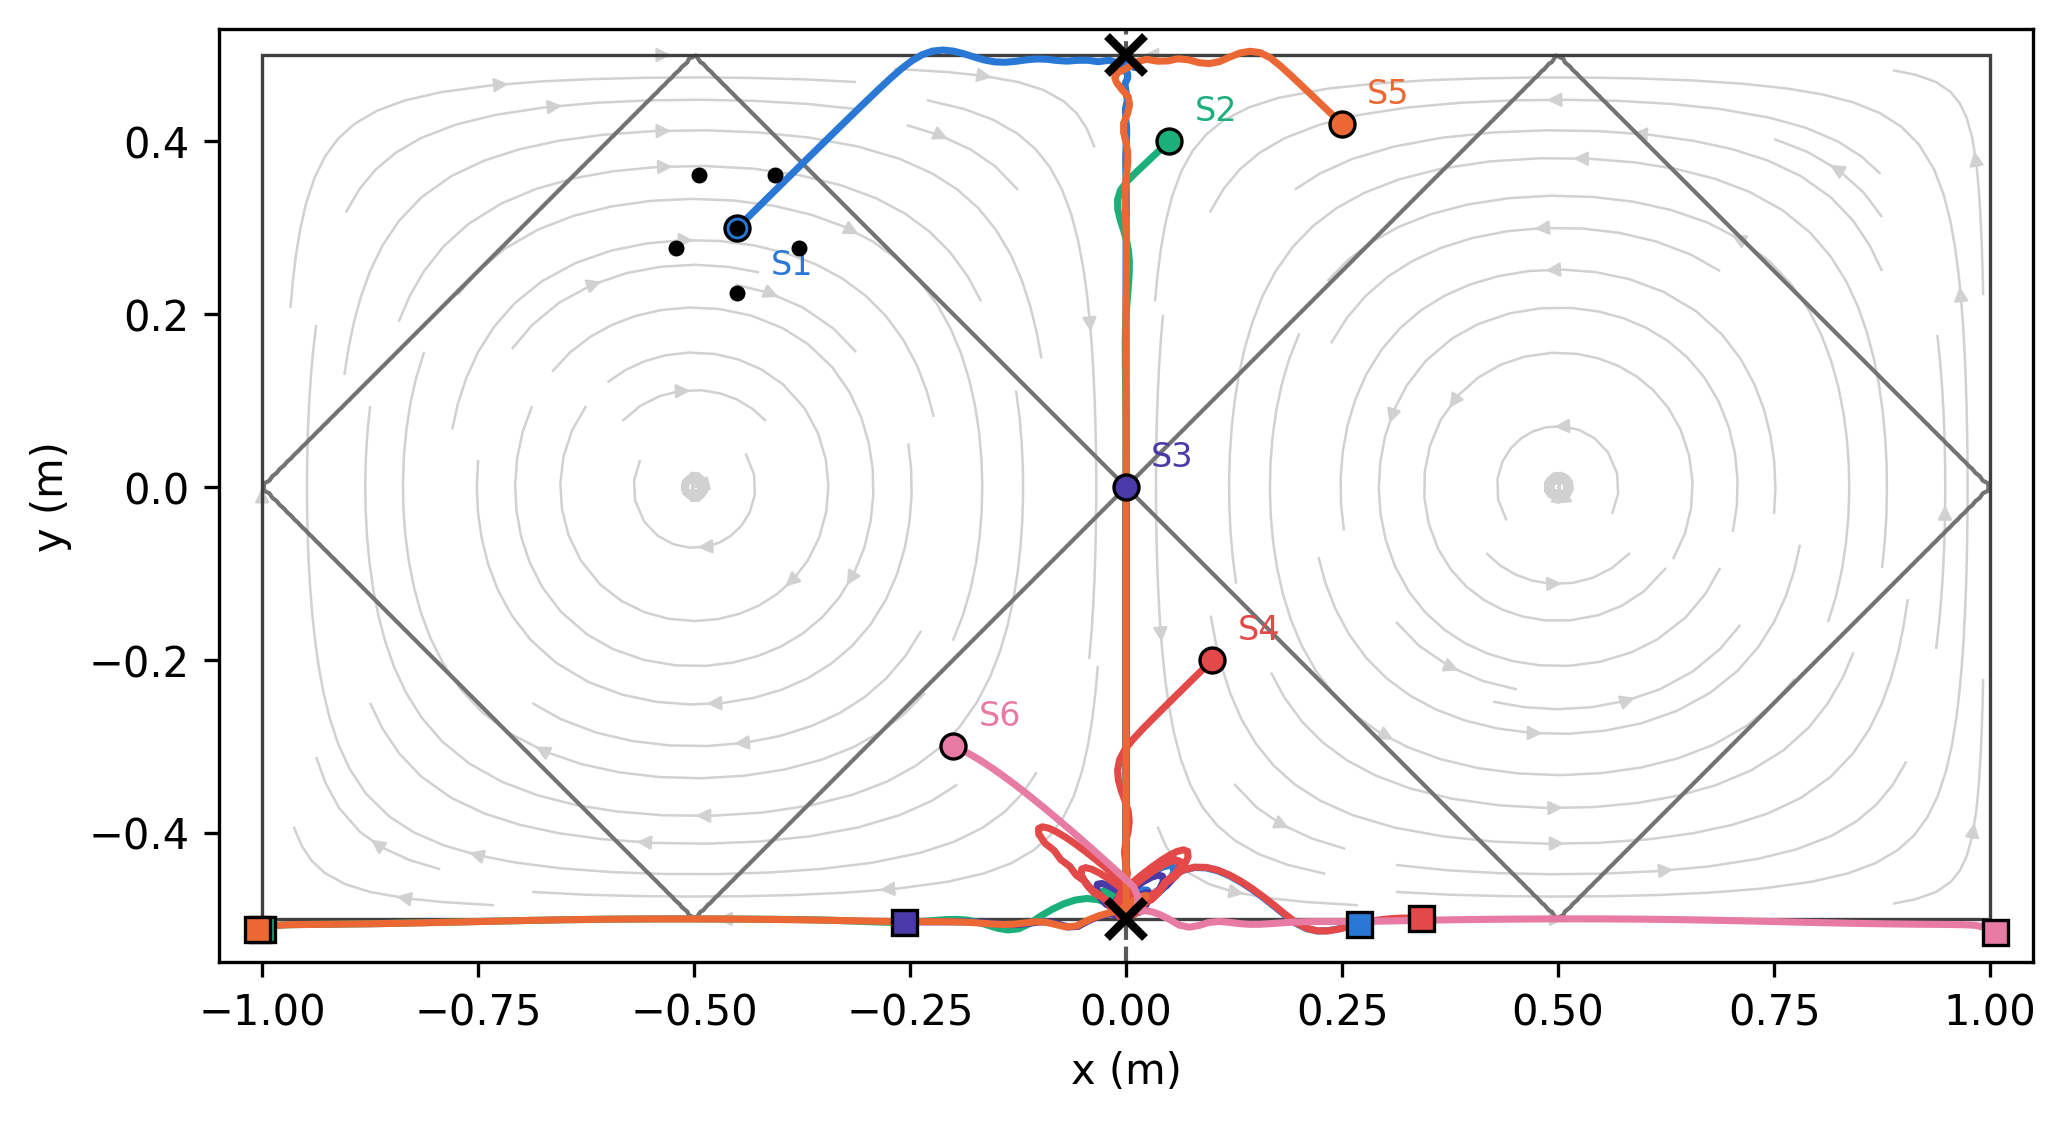
\includegraphics[width=0.45\textwidth]{figures/separatrix_trajectories.png}
    % TODO: plot cluster centroid trajectories from a grid of initial conditions
    % (at sigma_uv = 0). Overlay the double-gyre streamlines, the separatrix
    % (x=0), and the two saddle points. Use color to indicate time.
    \caption{Separatrix tracker (Logic C) centroid trajectories from a
    $5 \times 5$ grid of initial conditions, noise-free case. Final positions
    are marked with $\bullet$. The separatrix at $x = 0$ is shown as a dashed
    line.}
    \label{fig:sep_trajectories}
\end{figure}

\begin{figure}[!t]
    \centering
    
\includegraphics[width=0.45\textwidth]{figures/separatrix_success_rate.png}
    % TODO: heatmap of success rate over the (sigma_uv, sigma_p) grid
    % for the separatrix controller.
    \caption{Success rate of the separatrix tracker over the
    $(\sigma_{uv}, \sigma_p)$ sweep. Each cell is the fraction of 200 trials
    that achieved time-to-band within 200 steps without formation collapse.}
    \label{fig:sep_success}
\end{figure}

% TODO: report separatrix controller results:
% (1) Convergence from nominal initial conditions (noise-free).
% (2) Mode distribution (fraction of time in FLOW / Logic A / Logic B).
% (3) Success rate heatmap. At what noise level does success rate degrade?
% (4) Mean and 95th percentile tracking error |x_c| over the tracking phase.

\subsection{Okubo-Weiss Boundary Tracker Simulation Results}

\begin{figure}[!t]
    \centering
    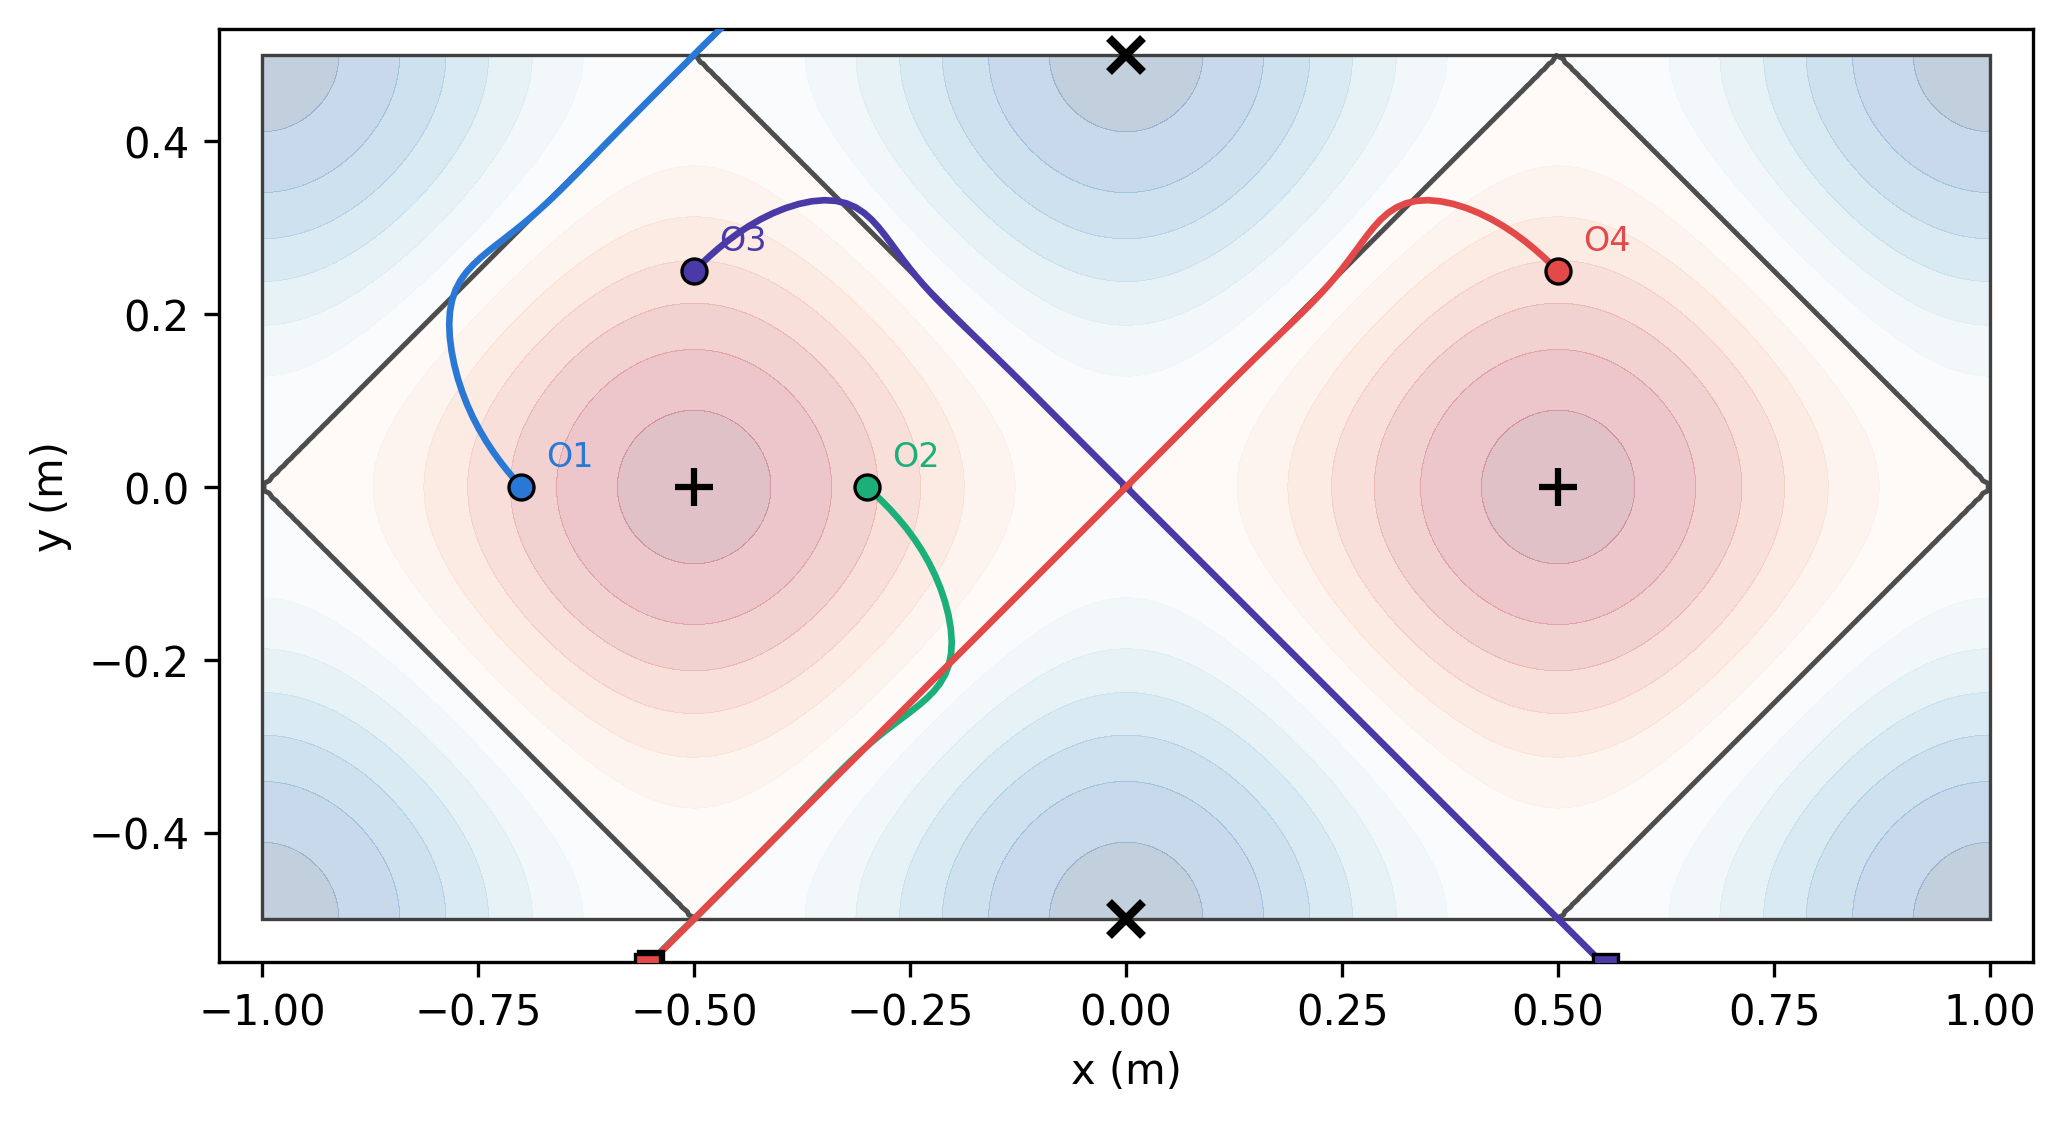
\includegraphics[width=0.45\textwidth]{figures/ow_trajectories.png}
    % TODO: plot OW controller centroid trajectories overlaid on the
    % det(J)=0 boundary. Use color to show time. Show convergence to the
    % boundary and tangential drift.
    \caption{Okubo-Weiss boundary tracker centroid trajectories from a
    $5 \times 5$ grid of initial conditions, noise-free case. The
    $\det(\mathbf{J}) = 0$ boundary is shown as a bold curve.}
    \label{fig:ow_trajectories}
\end{figure}

\begin{figure}[!t]
    \centering
    
\includegraphics[width=0.45\textwidth]{figures/ow_success_rate.png}
    % TODO: heatmap of success rate over (sigma_uv, sigma_p) for OW controller.
    \caption{Success rate of the Okubo-Weiss boundary tracker over the
    $(\sigma_{uv}, \sigma_p)$ sweep.}
    \label{fig:ow_success}
\end{figure}

% TODO: report OW controller results:
% (1) Convergence to det(J)=0 from nominal initial conditions.
% (2) Tangential drift behavior: does the cluster orbit the gyre center?
% (3) Success rate heatmap. Compare with separatrix controller.
% (4) Mean and 95th percentile |D(p_c)| over tracking phase.

\subsection{Comparison of the Two Controllers}

\begin{figure}[!t]
    \centering
    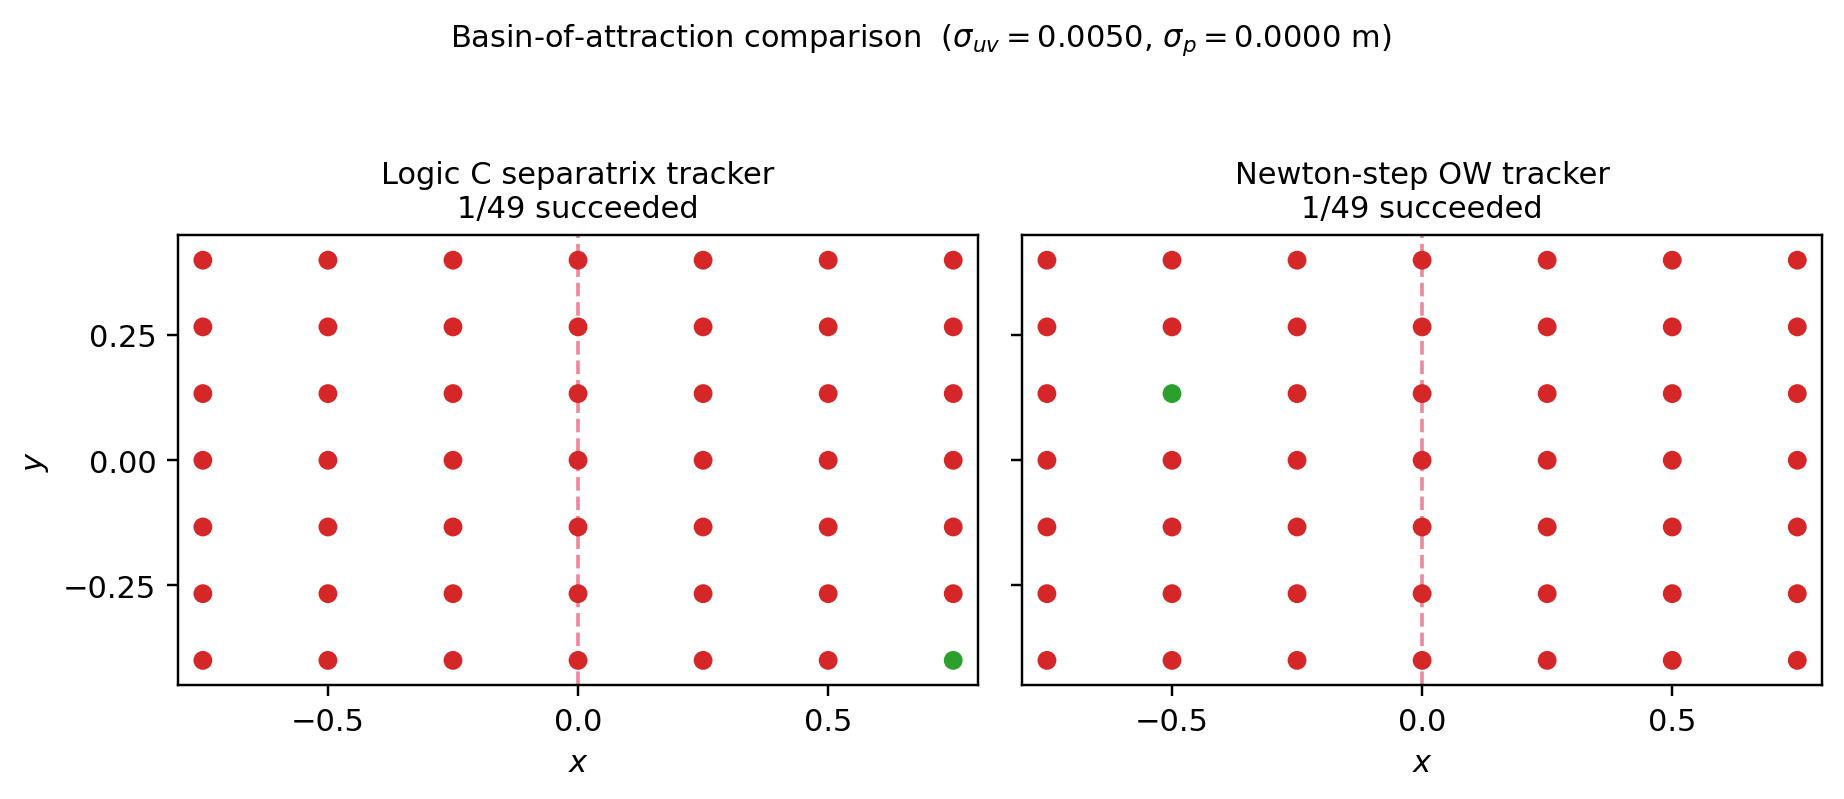
\includegraphics[width=0.45\textwidth]{figures/controller_comparison.png}
    % TODO: side-by-side basin-of-attraction plots for both controllers
    % at the same sigma_uv level.
    \caption{Basin-of-attraction comparison: fraction of trials that
    converge from each initial centroid cell, for the separatrix tracker
    (left) and the OW boundary tracker (right), at
    $\sigma_{uv} = $~% TODO: insert noise level.
    }
    \label{fig:comparison}
\end{figure}

% TODO: discuss which controller has a larger basin of attraction, which is
% more sensitive to noise, and the fundamental difference in what each tracks
% (a manifold vs a closed curve).


% ---------------------------------------------------------------------------
\section{Discussion}
\label{sec:discussion}

\subsection{Implications for Distributed Eulerian-Structure Following}

% TODO: 4-6 sentences. Discuss: (1) the finding that a six-robot formation
% can recover enough second-order spatial information of a vector field to
% locate and track Eulerian structures without global field knowledge;
% (2) the role of the det(J) landscape (the trench) as a navigation
% target that is computable from local samples; (3) how the two controllers
% address complementary structures (a manifold and a closed boundary).

\subsection{Failure Modes}

% TODO: 4-6 sentences. Cover:
% (1) Estimator ill-conditioning when the formation collapses toward a
%     degenerate configuration (det(Phi) small); propose formation-shape
%     maintenance as mitigation.
% (2) Mode-switching chatter in the separatrix controller when the
%     centroid oscillates across the FLOW-band boundary; discuss the
%     role of the dimensionless threshold eps_dim in damping this.
% (3) Tangential drift in the OW controller can carry the cluster away
%     from the domain boundaries; note this is a simulation artifact
%     (infinite domain).


% ---------------------------------------------------------------------------
\section{Limitations}
\label{sec:limitations}

This paper restricts attention to the static double gyre ($\varepsilon = 0$).
In the time-varying case ($\varepsilon > 0$) the separatrix becomes a
material curve that evolves with the flow, and the det$(\mathbf{J}) = 0$
boundary shifts in time; tracking either structure would require adapting
the control law to account for the flow unsteadiness. This extension is
left to future work.

Results are presented for a single field family (the double gyre). Whether
the separatrix tracker and OW boundary tracker generalize to other fields
with saddle-like or rotation-dominated regions is not addressed here,
though the estimation framework (Section~\ref{sec:estimation}) applies
to any smooth planar vector field.

All results are from simulation only. Hardware validation on the Decabot
testbed is not reported in this paper; it is planned as a follow-on study.


% ---------------------------------------------------------------------------
\section{Future Work}
\label{sec:future}

Direct extensions of this work include:
\begin{itemize}
    \item \textbf{Time-varying double gyre.} Extending the controllers to
          the $\varepsilon > 0$ case by adding a time-derivative correction
          term to the navigation primitive.
    \item \textbf{Online formation reshaping.} Adapting the pair lengths
          $(L_k)$ and the SAS parameters to improve the conditioning of
          $\boldsymbol{\Phi}$ when the cluster is near a degenerate
          configuration.
    \item \textbf{Hardware deployment.} Validating both controllers on the
          Decabot testbed using the OptiTrack motion-capture system. The
          separatrix and Okubo-Weiss boundaries can be represented by a
          vector field emitted by an on-board computer and sampled by
          the robots' onboard sensors.
    \item \textbf{Extension to 3D.} Generalizing the quadratic estimator
          to three-dimensional fields, which would require at least 10 robots
          per component for full cubic determination, or a reduced-order
          estimator with different assumptions.
\end{itemize}


% ---------------------------------------------------------------------------
\section{Conclusion}
\label{sec:conclusion}

This paper presented a distributed framework for navigating a six-robot
formation along two Eulerian structural boundaries of the double gyre: the
separatrix and the Okubo-Weiss ($\det(\mathbf{J}) = 0$) boundary. A quadratic
estimator using simultaneous measurements from the six robots recovers the
Jacobian, its determinant, gradient, and Hessian at the cluster centroid with
no prior field knowledge. Two parallel adaptive controllers were derived, each
with a Lyapunov stability certificate. Monte Carlo simulation over a
two-dimensional noise sweep quantified the noise robustness of both
controllers.

% TODO: replace the sentences above with specific results once Section IX
% is filled in (success rates, tracking error bounds, noise thresholds).


\appendices

% ---------------------------------------------------------------------------
\section{Double-Gyre Analytic Forms}
\label{app:analytic}

For the static double gyre with $A = 0.1$, $x_f = x + 1$,
$y_f = y + 0.5$, define $s_x = \sin(\pi x_f)$, $c_x = \cos(\pi x_f)$,
$s_y = \sin(\pi y_f)$, $c_y = \cos(\pi y_f)$. The field is
$u = -\pi A s_x c_y$, $v = \pi A c_x s_y$.

The Jacobian entries are
\begin{equation}
    \frac{\partial u}{\partial x} = -\pi^2 A c_x c_y, \quad
    \frac{\partial u}{\partial y} =  \pi^2 A s_x s_y,
\end{equation}
\begin{equation}
    \frac{\partial v}{\partial x} = -\pi^2 A s_x s_y, \quad
    \frac{\partial v}{\partial y} =  \pi^2 A c_x c_y.
\end{equation}
Hence
\begin{equation}
    \det(\mathbf{J}) = -\pi^4 A^2 c_x^2 c_y^2 - \pi^4 A^2 s_x^2 s_y^2
                     = -\pi^4 A^2 \bigl(c_x^2 c_y^2 + s_x^2 s_y^2\bigr).
                     \label{eq:det_analytic}
\end{equation}
Note that $\det(\mathbf{J}) \leq 0$ everywhere in the domain: the double gyre
has no rotation-dominated regions when evaluated in the world frame under this
convention. The $\det(\mathbf{J}) = 0$ contour requires
$c_x^2 c_y^2 + s_x^2 s_y^2 = 0$, which in the world frame occurs when...

% TODO: complete the det(J)=0 condition derivation. Use trig identities to
% simplify c_x^2 c_y^2 + s_x^2 s_y^2 = (1/2)(1 + cos(2*pi*x_f)*cos(2*pi*y_f)).
% Set equal to zero and find the zero curves. Verify against the numerical
% contour in Fig. 2.

The gradient components are
\begin{equation}
    \frac{\partial \det(\mathbf{J})}{\partial x} =
    % TODO: derive analytically from eq:det_analytic.
    \label{eq:grad_det_analytic_x}
\end{equation}
\begin{equation}
    \frac{\partial \det(\mathbf{J})}{\partial y} =
    % TODO: derive analytically.
    \label{eq:grad_det_analytic_y}
\end{equation}

The Hessian entries $\partial^2 \det(\mathbf{J}) / \partial x^2$,
$\partial^2 \det(\mathbf{J}) / \partial x \partial y$,
$\partial^2 \det(\mathbf{J}) / \partial y^2$ follow by differentiating the
gradient expressions above.

% TODO: complete the Hessian derivation and write out the three entries.

The Okubo-Weiss parameter is $Q = -\det(\mathbf{J})$, so $Q \geq 0$
throughout the domain (all regions are strain-dominated or neutral under
this sign convention). The $Q = 0$ contour is the same as the
$\det(\mathbf{J}) = 0$ contour.

% TODO: verify the sign interpretation and cross-check with the literature.
% Confirm whether the convention matches Okubo (1970) and Weiss (1991).


% ---------------------------------------------------------------------------
\section{Pentagon Cluster Kinematics}
\label{app:kinematics}

\subsection{Forward Kinematics}

The pentagon-of-pairs cluster has 6 robots indexed $i = 1, \ldots, 6$, arranged
as three pairs. Pair $k$ ($k = 1, 2, 3$) consists of robots $2k-1$ and $2k$.
The midpoint of pair $k$ is $\mathbf{m}_k = (\mathbf{p}_{2k-1} +
\mathbf{p}_{2k})/2$. The three midpoints form a triangle; the centroid of that
triangle is $\mathbf{p}_c = (\mathbf{m}_1 + \mathbf{m}_2 + \mathbf{m}_3)/3$.

The SAS parameters of the midpoint triangle are defined as in the three-robot
case: $p_1 = \|\mathbf{m}_2 - \mathbf{m}_1\|$, $q_1 = \|\mathbf{m}_3 -
\mathbf{m}_2\|$, and $\beta_1$ is the interior angle at $\mathbf{m}_2$.
The cluster heading $\theta_c = \text{atan2}(m_{2,y} - m_{1,y},
m_{2,x} - m_{1,x})$.

Each pair is described by its half-length $L_k/2$ and orientation angle
$\psi_k$, so the two robots in pair $k$ are at $\mathbf{m}_k \pm (L_k/2)
(\cos\psi_k, \sin\psi_k)^\top$.

The full 12-state cluster configuration is
$(x_c, y_c, \theta_c, p_1, \beta_1, q_1, L_2, \psi_2, L_3, \psi_3,
L_4, \psi_4)$, where pair 1 uses $L_1$ fixed and $\psi_1 = \theta_c$ by
convention.

\subsection{Inverse Kinematics}

Given the 12-state cluster configuration, the six robot positions are recovered
by:
\begin{enumerate}
    \item Constructing the midpoint triangle from $(p_1, \beta_1, q_1)$ in
          a local frame (following the same procedure as the three-robot
          cluster in Appendix B of [6]).
    \item Rotating and translating to the global frame using $\theta_c$,
          $x_c$, $y_c$.
    \item Placing each pair of robots by offsetting from the midpoint along
          $(\cos\psi_k, \sin\psi_k)$ by $L_k/2$ in each direction.
\end{enumerate}

\subsection{Inverse Kinematic Jacobian}

The $12 \times 12$ inverse kinematic Jacobian maps desired cluster state
velocities $\dot{\boldsymbol{\xi}}$ to robot velocity commands
$(\dot{x}_1, \dot{y}_1, \ldots, \dot{x}_6, \dot{y}_6)^\top$:
\begin{equation}
    \begin{bmatrix} \dot{x}_1 \\ \dot{y}_1 \\ \vdots \\
    \dot{x}_6 \\ \dot{y}_6 \end{bmatrix}
    =
    \mathbf{J}_c^{-1}
    \begin{bmatrix} \dot{x}_c \\ \dot{y}_c \\ \dot{\theta}_c \\
    \dot{p}_1 \\ \dot{\beta}_1 \\ \dot{q}_1 \\
    \dot{L}_2 \\ \dot{\psi}_2 \\ \dot{L}_3 \\ \dot{\psi}_3 \\
    \dot{L}_4 \\ \dot{\psi}_4 \end{bmatrix},
    \label{eq:inv_kin_jac}
\end{equation}
where $\mathbf{J}_c^{-1}$ is a $12 \times 12$ matrix of partial derivatives
$\partial (x_i, y_i) / \partial \xi_j$ computed analytically from the inverse
kinematics. The explicit entries are omitted here for brevity; the
implementation is in \textit{pentagon\_kinematics.py}.


% ---------------------------------------------------------------------------
\begin{thebibliography}{99}

\bibitem{1} G. Haller and G. Yuan, "Lagrangian coherent structures and mixing
in two-dimensional turbulence," \textit{Physica D: Nonlinear Phenomena},
vol. 147, no. 3-4, pp. 352--370, 2000.

\bibitem{2} T. Peacock and G. Haller, "Lagrangian coherent structures: The
hidden skeleton of fluid flows," \textit{Physics Today}, vol. 66, no. 2,
pp. 41--47, 2013.

\bibitem{3} S. C. Shadden, F. Lekien, and J. E. Marsden, "Definition and
properties of Lagrangian coherent structures from finite-time Lyapunov
exponents in two-dimensional aperiodic flows," \textit{Physica D}, vol. 212,
no. 3-4, pp. 271--304, 2005.

\bibitem{4} R. T. McDonald, C. A. Kitts, and M. A. Neumann, "Navigation of
scalar fronts with multirobot clusters in simulation and experiment,"
\textit{IEEE Systems Journal}, vol. 14, no. 3, pp. 3755--3766, 2020.

\bibitem{5} C. A. Kitts, R. T. McDonald, and M. A. Neumann, "Adaptive
navigation control primitives for multirobot clusters: Extrema finding,
contour following, ridge/trench following, and saddle point station keeping,"
\textit{IEEE Access}, vol. 6, pp. 17625--17642, 2018.

\bibitem{6} C. Waight and C. A. Kitts, "Adaptive navigation of multirobot
systems to critical points in 2D vector fields," \textit{IEEE/ASME Transactions
on Mechatronics}, % TODO: add volume, issue, page range, year once published.

\bibitem{7} A. Okubo, "Horizontal dispersion of floatable particles in the
vicinity of velocity singularities such as convergences," \textit{Deep-Sea
Research}, vol. 17, no. 3, pp. 445--454, 1970.

\bibitem{8} J. Weiss, "The dynamics of enstrophy transfer in two-dimensional
hydrodynamics," \textit{Physica D: Nonlinear Phenomena}, vol. 48, no. 2-3,
pp. 273--294, 1991.

\bibitem{9} B.-L. Hua and P. Klein, "An exact criterion for the stirring
properties of nearly two-dimensional turbulence," \textit{Physica D}, vol. 113,
no. 1, pp. 98--110, 1998.

\bibitem{10} P. Ögren, E. Fiorelli, and N. E. Leonard, "Cooperative control
of mobile sensor networks: Adaptive gradient climbing in a distributed
environment," \textit{IEEE Transactions on Automatic Control}, vol. 49, no. 8,
pp. 1292--1302, 2004.

\bibitem{11} L. Briñón-Arranz, A. Renzaglia, and L. Schenato, "Multirobot
symmetric formations for gradient and Hessian estimation with application to
source seeking," \textit{IEEE Transactions on Robotics}, vol. 35, no. 3,
pp. 782--789, 2019.

\bibitem{12} C. A. Kitts and I. Mas, "Cluster space specification and control
of mobile multirobot systems," \textit{IEEE/ASME Transactions on Mechatronics},
vol. 14, no. 2, pp. 207--218, 2009.

\bibitem{13} T. Adamek, C. A. Kitts, and I. Mas, "Gradient-based cluster space
navigation for autonomous surface vessels," \textit{IEEE/ASME Transactions on
Mechatronics}, vol. 20, no. 2, pp. 506--518, 2014.

\bibitem{14} M. Michini, M. A. Hsieh, E. Forgoston, and I. B. Schwartz,
"Robotic tracking of coherent structures in flows," \textit{IEEE Transactions
on Robotics}, vol. 30, no. 3, pp. 593--603, 2014.

\bibitem{15} D. Kularatne and M. A. Hsieh, "Tracking attracting manifolds in
flows," \textit{Autonomous Robots}, vol. 41, no. 8, pp. 1575--1588, 2017.

\bibitem{16} G. Knizhnik, P. Li, X. Yu, and M. A. Hsieh, "Flow-based control
of marine robots in gyre-like environments," in \textit{Proc. 2022 Int. Conf.
on Robotics and Automation (ICRA)}, pp. 3047--3053, 2022.

% TODO: add any additional references as needed (Haller 2015 coherent structure
% review, Hunt Q-criterion 1988, additional cluster space references, etc.).

\end{thebibliography}


\begin{IEEEbiography}[{
\includegraphics[width=1in,height=1.25in,clip,keepaspectratio]{figures/cwaight.jpg}}]{Christopher Waight}
% TODO: insert bio.
\end{IEEEbiography}

\begin{IEEEbiography}[{
\includegraphics[width=1in,height=1.25in,clip,keepaspectratio]{figures/ckitts.jpg}}]{Christopher A. Kitts}
% TODO: insert bio.
\end{IEEEbiography}

\end{document}
